% ============================================================================
% main.tex --- Master manuscript file
% Title: Asymmetric Loss Modulation Resolves the Voting Ensemble Paradox
%        in Learned Context-Pruning Ensembles
% Target venue: ICLR 2027 (double-blind) ; arXiv preprint host
% Lead thesis: Voting Ensemble Paradox + 3.0x asymmetric loss modulation fix
% Frame: Loop Engineering paradigm (Osmani 2026 ; Greyling 2026 ; LangChain 2026)
% Substrate: kompress-v8 (PeetPedro/kompress-v8) + LoopKit (peterlodri-sec/loopkit)
% Dataset: ultrawhale-dogfood (PeetPedro/ultrawhale-dogfood)
% Logs: https://pocoo.vaked.dev
% ----------------------------------------------------------------------------
% Build:  pdflatex main && bibtex main && pdflatex main && pdflatex main
% ============================================================================
\documentclass[10pt,letterpaper]{article}

% --- If the ICLR style file is available, swap the line below for the venue
%     style and remove the manual geometry. For anonymized double-blind
%     submission use:  \usepackage{iclr2027_conference}
\usepackage[margin=1in]{geometry}

% --- Core packages ---
\usepackage{amsmath,amssymb,amsthm}
\usepackage{mathtools}
\usepackage{booktabs}
\usepackage{multirow}
\usepackage{array}


\usepackage{graphicx}
\usepackage{xcolor}
% microtype omitted — font expansion unavailable in this TeX Live
\usepackage{url}
\usepackage[round,authoryear]{natbib}
\usepackage{hyperref}
\hypersetup{colorlinks=true,linkcolor=blue!60!black,citecolor=teal!60!black,urlcolor=blue!60!black}

% --- Theorem environments ---
\newtheorem{theorem}{Theorem}
\newtheorem{proposition}{Proposition}
\newtheorem{corollary}{Corollary}
\newtheorem{lemma}{Lemma}
\newtheorem{definition}{Definition}
\newtheorem{assumption}{Assumption}
\newtheorem{remark}{Remark}

% --- Custom notation shortcuts ---
\newcommand{\I}{\mathbb{I}}          % indicator
\newcommand{\R}{\mathbb{R}}
\newcommand{\E}{\mathbb{E}}
\renewcommand{\Pr}{\mathbb{P}}
\renewcommand{\vec}[1]{\boldsymbol{#1}}
\newcommand{\Lcrit}{\mathcal{L}_{\mathrm{crit}}}
\newcommand{\Lbase}{\mathcal{L}_{\mathrm{base}}}

% ============================================================================
% Metadata
% ============================================================================
\title{Asymmetric Loss Modulation Resolves the Voting Ensemble Paradox\\
       in Learned Context-Pruning Ensembles}

% Open-science preprint header (swap with Anonymous Authors block below for double-blind OpenReview submission).
\author{Peter Lodri%
  \thanks{Independent, community-funded research. Decentralized open-source
  funding model: community-council-guided donations; no institutional grant.
  Open-science preprint (target venue: ICLR 2027).}%
  \\[2pt]
  \texttt{https://pocoo.vaked.dev \quad https://github.com/8b-is/longrun-eval-kompress}}

% --- Anonymized block for double-blind submission (uncomment and redact URLs) -
% \author{Anonymous Authors\\
%         Paper under double-blind review\\
%         \texttt{anonymous}}
% ----------------------------------------------------------------------------

\date{}

\begin{document}
\maketitle

% ============================================================================
% Abstract
% ============================================================================
\begin{abstract}
Learned context pruning improves long-context agent efficiency but introduces
a failure mode we term the \emph{Voting Ensemble Paradox}: when multiple
compression checkpoints with asymmetric training-data floors are combined
under $k$-of-$N$ voting---a common safety-gating configuration---the
ensemble's eviction decision collapses, stratum by stratum, to the
per-stratum $k$-th weakest voter. The resulting global operating point is
Pareto-dominated by the frontier of any single strong checkpoint and, when
the weakest voter differs across strata, is occupied by no individual model.
We formalize this collapse via a conditional-probability proof over
indicator functions and trace it to per-stratum monotone-rejection
refinement across asymmetric floors. As a corrective, we introduce three
complementary mechanisms: \textbf{(A)} a $3.0\times$ weighted
cross-entropy penalty on critical-syntactic tokens (signal names, file
paths, exit codes) during fine-tuning---the critical-token penalty; \textbf{(B)}
a post-inference regex override that surgically force-keeps must-keep
tokens at deployment; and \textbf{(C)} a self-labeling loop that uses
A+B as an oracle to relabel the training data, internalizing B so the
inference override becomes redundant. We instantiate the method in
\textbf{kompress-v8}, a 149M-parameter dual-head ModernBERT (token
classifier + Span CNN) trained via C3 self-distillation
(Collect--Curate--Compress) with a Qwen2.5-7B teacher on real agent tool
outputs, on the \textbf{ultrawhale-dogfood} silver-label corpus, and
orchestrated by \textbf{LoopKit}, an open-source four-phase autonomous state
machine realizing the recursive loop-stacking taxonomy of Loop Engineering
\citep{osmani2026loop,greyling2026loop,langchain2026loops}. Empirically, on the 8-prompt adversarial \texttt{heretic} benchmark,
mechanism~A raises must-keep survival to $0.942$ (macro-averaged, no
override; $0.911$ on the initial unnormalized evaluation split, lifted by
mechanism~B to $0.965$, $\mathit{override\_delta}{=}{+}0.054$), while
mechanism~C (v4) internalizes the override to reach $0.967$ with
$\mathit{override\_delta}{=}0.000$ ($0.961\to0.965$ under the Table~\ref{tab:override}
protocol). On the expanded 32-prompt benchmark, the production model v8
reaches $0.955$ ($+0.012$ over v4's $0.943$) at $15\%$ compression
($\mathit{keep\_rate}{=}0.854$) with $\mathit{override\_delta}{=}0.000$ and
agent $\mathit{mk\_in\_ref}{=}1.000$ under the deployment override. A
$\lambda\in\{3,5,10\}$ ablation maps the Pareto frontier:
$\lambda{=}10$ achieves $0.972$ heretic at $2.8\%$ compression, while
$\lambda{=}3$ (v8) is the production sweet spot at $15\%$ compression. Across
17 models in the lineage (v2-base, v3.3 control, and 15 LoopKit outer-loop
checkpoints v3--v17), 8 teachers, and 4 architectures, the dominant signal is
label quality---not model capacity or data quantity. On the 8-prompt set, a
3-checkpoint majority ensemble ($k_{\mathrm{drop}}{=}2/3$) and drop-if-any
ensemble ($k_{\mathrm{drop}}{=}1/3$) both regress to $0.931$---a $0.031$
paradox collapse below the best single model ($0.9618$ unrounded)---which a
higher-floor ensemble avoids. Against external baselines on the 8-prompt set,
kompress-v8 achieves $0.993$ $\mathit{exact\_keep\_pct}$ (with production
override; $0.967$ pure neural v4) vs.\ LLMLingua-2's $0.867$ and TextRank's
$0.599$.
\end{abstract}

% ============================================================================
% Body --- modular via \include
% ============================================================================
% introduction.tex --- Section 1
\section{Introduction}
\label{sec:introduction}

Long-context agents increasingly rely on automated context pruning to remain
within effective working windows. The pruning decision, however, is not
semantically neutral: it removes tokens, and tokens constitute the vocabulary
in which an agent can reason. A downstream agent cannot
reason about a signal name, file path, or exit code that has been evicted from
its context; token eviction is therefore an act of \emph{representational
impoverishment}, and its harm concentrates on the \emph{critical-syntactic}
token class---identifiers, paths, exit codes, delimiters---that anchors agent
tool-use and control flow. (We note the parallel to the linguistic-relativity
hypothesis---that the vocabulary available to a reasoner shapes what it can
reason about---without claiming a deeper connection.)

This framing is sharpened by the emergence of \emph{Loop Engineering}
\citep{osmani2026loop}, the mid-2026 shift from hand-crafting prompts to
designing autonomous systems that discover, execute, verify, and improve on a
schedule or until a goal is met. As articulated by Osmani and echoed by
Cherny and Steinberger, the engineer's role migrates from operator to system
designer \citep{osmani2026oreilly}; Greyling provides the reference
implementation and operational playbook (persistent \texttt{STATE.md}
tracking, \texttt{loop-cost} token gating, \texttt{loop-run-log.md}
conventions) \citep{greyling2026loop}; and LangChain formalizes a four-tier
stacked-loop taxonomy (agent, verification, event-driven, hill-climbing)
\citep{langchain2026loops}. We applied these patterns to the kompress problem
in \citet{lodri2026loopapplied}, mapping Osmani's five building blocks and
Anthropic's agent patterns to a real compression fine-tuning pipeline. In this
paradigm the pruning model is not a static
preprocessing step but a component inside a recursive control structure, and
its errors \emph{compound} across loop iterations---a single false eviction in
one cycle can starve every subsequent cycle of the context needed to recover.
In this paper we focus on \emph{intrinsic critical-token preservation}
($\mathit{exact\_keep\_pct}$) and token compression rate
($1-\mathit{keep\_rate}$) on single-turn tool and technical outputs as a
controlled, deterministic proxy for multi-cycle context fidelity, leaving
end-to-end multi-turn agent task completion benchmarks to future work.

\subsection{Origin: the vaked and ultrawhale outer loops}

The research in this paper emerged from two outer-loop systems that preceded
it. \textbf{ultrawhale}\footnote{\url{https://github.com/peterlodri-sec/ultrawhale}}
is a self-building coding agent (150 blocks, 7 recursions, 14 protocols) whose
dogfeed loop generates Q\&A training data by querying free LLMs every ten
seconds and depositing the results as a living dataset on HuggingFace
(\texttt{PeetPedro/ultrawhale-dogfood}). \textbf{vaked} is the broader
capability-language and infrastructure framework within which ultrawhale
operates. The entire ultrawhale project (v1.0.0$\to$v100.1.0) was
developed via loop engineering in 150 blocks, demonstrating that the outer
loop produced both the idea and the dataset for this paper. This paper is
an inner loop of that broader program: the pruning model that makes the
outer loops cheaper to
 run by compressing the context they accumulate. The full experiment log is
 published at \url{https://pocoo.vaked.dev}---a chronological registry of
 every training run, evaluation, and dead end
 \citep{lodri2026sapirwhorf,lodri2026selflabeling,lodri2026heretic,
 lodri2026silverlabel,lodri2026loopkit,lodri2026loopshipped}.

\subsection{The Voting Ensemble Paradox}

A natural safety pattern in such systems is to gate pruning decisions through
a \emph{multi-checkpoint voting ensemble}: combining $N$ compression
checkpoints under a $k_{\mathrm{drop}}$-of-$N$ eviction rule
(Definition~\ref{def:kofn}), where at least $k_{\mathrm{drop}}$ voters must
vote to evict a token before it is dropped. Intuitively, ensembling multiple
checkpoints---whether via a strict \emph{unanimity-to-keep} (AND-keep,
$k_{\mathrm{drop}}{=}1$, where any voter's drop evicts) or a \emph{majority}
gate ($k_{\mathrm{drop}}{=}2$ of $3$)---is expected to stabilize decisions across
models. We show that when checkpoints are trained on \emph{asymmetric data
floors}, this intuition inverts for every $k_{\mathrm{drop}} < N$.

Because weaker checkpoints (trained on lower-quality or lower-quantity silver
labels) evict more aggressively, and because this aggression is
\emph{stratum-dependent}---each checkpoint is weakest on the stratum its
training set under-represented---$k_{\mathrm{drop}}$-of-$N$ voting pins each
stratum's eviction decision to its $k_{\mathrm{drop}}$-th most aggressive
voter (for AND-keep $k_{\mathrm{drop}}{=}1$, the single weakest voter; for
majority $k_{\mathrm{drop}}{=}2$ of $3$, the per-stratum median). Under
AND-keep ($k_{\mathrm{drop}}{=}1$), the ensemble's eviction set becomes the
stratum-wise union of each weakest voter's rejections: a global operating
point whose must-keep recall is dominated by any single strong checkpoint and,
when the weakest voter differs across strata, is \emph{occupied by no
individual model}. Adding a stronger voter cannot rescue a stratum where $k_{\mathrm{drop}}$
weaker voters still agree to evict. We call this the \textbf{Voting Ensemble
Paradox}.

\subsection{Contributions}

This paper makes the following contributions:

\begin{enumerate}
  \item \textbf{Formalization of the Voting Ensemble Paradox.} We prove
        (Theorem~\ref{thm:paradox}) that under $k_{\mathrm{drop}}{=}1$
        (AND-keep) voting, per-stratum false-eviction rates are bounded below
        by the worst voter for arbitrary checkpoints and equal the per-stratum
        weakest voter's under monotone-rejection refinement
        (Definition~\ref{def:monotone}), generalizing to the $k_{\mathrm{drop}}$-th
        order statistic under a per-stratum nested chain (Remark~\ref{rem:kofn})
        and yielding a stratum-wise recall collapse (Corollary~\ref{cor:pareto}).
  \item \textbf{Three complementary correctives.} We introduce and
        separate: (A) a $3.0\times$ weighted cross-entropy penalty on
        critical-syntactic tokens during fine-tuning---the critical-token
        penalty; (B) a post-inference subword-window regex override that
        surgically force-keeps must-keep tokens at deployment; and (C) a
        self-labeling loop that uses A+B as an oracle to relabel and retrain,
        internalizing B so the inference override becomes redundant.
  \item \textbf{kompress-v8.} Building on the 149M-parameter dual-head
        ModernBERT (\texttt{chopratejas/kompress-v2-base}; token classifier +
        Span CNN) architecture, we formulate an asymmetric non-negative
        modulation gate between the two heads and fine-tune via C3
        self-distillation (Collect--Curate--Compress) with a Qwen2.5-7B
        teacher on real agent tool outputs. Across 17 models in the project
        lineage (v2-base, v3.3 control, and 15 LoopKit checkpoints v3--v17),
        8 teachers, and 4 architectures, the $\lambda\in\{3,5,10\}$ ablation
        maps the full Pareto frontier of must-keep recall vs.\ compression. v8
        at $\lambda{=}3$ is the production sweet spot.
  \item \textbf{LoopKit substrate.} An open-source four-phase autonomous
        state machine (Plan, Execute, Evaluate, Decide) with an asynchronous
        SQLite state kernel and an LLM Council operator, instantiating the
        LangChain four-tier loop stack \citep{lodri2026loopkit}.
  \item \textbf{CI agent suite.} Six automated agents
        (\texttt{citation-guard}, \texttt{metric-watchdog},
        \texttt{changelog-gen}, \texttt{hf-card-sync}, \texttt{latex-guard},
        \texttt{doc-sync}) that enforce documentation--code consistency,
        citation validity, and metric stability on every push. The agents
        follow a layered abstraction (\texttt{CIAgent} base class, registry,
        CLI + MCP interface) and are advisory by design---they report
        pass/fail but never block the shipping loop.
  \item \textbf{Empirical validation.} On the 8-prompt \texttt{heretic} set,
        Mechanism~A reaches $0.942$ (macro-averaged, no override; $0.911$ on
        the initial Table~\ref{tab:override} split); Mechanism~B lifts v3
        $0.911\to0.965$ ($0.942\to0.969$ macro-averaged) and v4
        $0.961\to0.965$; Mechanism~C (v4) reaches $0.967$ with
        $\mathit{override\_delta}{=}0.000$. On the 32-prompt set, production
        model v8 reaches $0.955$ ($+0.012$ over v4's $0.943$) at $15\%$
        compression with agent $\mathit{mk\_in\_ref}{=}1.000$ under the
        override. A $\lambda\in\{3,5,10\}$ ablation maps the Pareto frontier
        ($0.955\to0.963\to0.972$ at $15\%\to3.7\%\to2.8\%$ compression). Both
        $k_{\mathrm{drop}}{=}2/3$ (majority) and $k_{\mathrm{drop}}{=}1/3$
        (drop-if-any) 3-checkpoint ensembles regress to $0.931$ on the 8-prompt
        set---a $0.031$ collapse below v4 ($0.9618$ unrounded)---confirming the
        paradox. Baselines (8-prompt set): kompress-v8 $0.993$ (with override;
        $0.967$ pure neural v4) vs.\ LLMLingua-2 $0.867$ vs.\ TextRank $0.599$
        vs.\ random $0.910$.
\end{enumerate}

\subsection{Paper structure}

Section~\ref{sec:related} situates the work among learned compression methods,
the Loop Engineering paradigm, and ensemble theory.
Section~\ref{sec:methodology} formalizes the paradox, derives the modulated
loss, and details the dual-head architecture.
Section~\ref{sec:evaluation} reports the empirical evaluation, including the
override/no-override ablation and external baselines.
Appendix~\ref{sec:loopkit} describes the LoopKit implementation as the
experimental substrate and its mapping to the four-tier loop taxonomy.
Section~\ref{sec:data} covers data availability, the decentralized funding
model, and acknowledgments. An interactive marimo companion with live paradox
simulation and baseline exploration is hosted at
\url{https://kompress.vaked.dev/notebook/}.

% related_work.tex --- Section 2
\section{Related Work}
\label{sec:related}

\subsection{Learned context pruning and prompt compression}
\label{sec:rw:compression}

Context pruning methods divide into prompt-level and training-based families.
\textbf{Selective Context} prunes lexical units via self-information
\citep{li2023selective}; \textbf{LLMLingua} and \textbf{LongLLMLingua}
introduce coarse-to-fine perplexity scoring and post-compression subsequence
recovery to mitigate entity corruption in long contexts
\citep{jiang2023llmlingua,jiang2024longllmlingua}; and \textbf{LLMLingua-2}
distills a GPT-4 compression oracle into a bidirectional token classifier
\citep{pan2024llmlingua2}. \textbf{AutoCompressors} recurrently summarize
context into summary tokens that condition subsequent generation
\citep{chevalier2023autocompressors}. \textbf{Gisting} trains a model to
compress prompts into a small set of gist tokens via cross-attention
\citep{mu2023gisting}. Classical unsupervised summarization
(\textbf{TextRank}; \citealp{mihalcea2004textrank}) provides a non-learned
floor. Our setting differs in three respects: (i) eviction targets
\emph{critical-syntactic} tokens (flags, paths, exit codes, hex addresses)
whose removal breaks agent tool-use rather than merely reducing fluency, with
Mechanism~B operating as a pre-eviction subword-window veto rather than post-hoc
string substitution; (ii) we fine-tune the dual-head ModernBERT + Span-CNN
architecture of \texttt{chopratejas/kompress-v2-base} with an asymmetric
modulation gate and $3.0\times$ critical-token loss; and (iii) we formalize and
empirically evaluate the \emph{ensemble behavior} of multiple pruners trained
on asymmetric floors, a regime prior methods do not address.

\subsection{Loop Engineering and autonomous agent loops}
\label{sec:rw:loopeng}

Loop Engineering denotes the shift from turn-by-turn prompting to designing
systems that prompt, verify, and improve agents autonomously
\citep{osmani2026loop}. Osmani identifies five building blocks---automations,
worktrees, skills, connectors, and sub-agents---plus an external memory spine,
echoing remarks by Cherny (Anthropic) and Steinberger (OpenClaw) that the
engineer's job is to write loops rather than prompts
\citep{osmani2026oreilly}. Greyling operationalizes this into a reference
repository with patterns and CLI tooling, introducing persistent
\texttt{STATE.md} state tracking, \texttt{loop-cost} token gating, and the
\texttt{loop-run-log.md} run-history convention \citep{greyling2026loop}.
LangChain formalizes the recursive structure as a four-tier stacked loop
model: (1) the agent loop, (2) a verification loop wrapping it with a grader,
(3) an event-driven loop connecting the agent to external triggers, and (4) a
hill-climbing loop that analyzes traces and rewrites the harness
\citep{langchain2026loops,langchain2026harness}. Our LoopKit system
(Appendix~\ref{sec:loopkit}) instantiates this four-tier stack and contributes
an asynchronous SQLite state kernel as the durable memory spine, with the
pruning ensemble operating inside the verification tier.

\subsection{Token importance and structured eviction}
\label{sec:rw:importance}

Modern bidirectional encoders such as \textbf{ModernBERT} provide the
long-context, memory-efficient backbone on which our pruner is built
\citep{warner2024modernbert}. Inherited from the open-source
\texttt{chopratejas/kompress-v2-base} adapter, the dual-head design---a token
classifier paired with a span CNN---separates \emph{per-token} eviction
decisions from \emph{span-level} coherence. We formalize the coupling between
heads via a non-negative asymmetric modulation gate (Section~\ref{sec:arch})
and pair it with a $3.0\times$ critical-token loss penalty (Section~\ref{sec:loss}),
extending the structured-eviction line by treating critical-syntactic token
classes as a protected subset rather than scoring all tokens uniformly.

\subsection{Ensembles, exchangeability, and the non-exchangeability gap}
\label{sec:rw:ensembles}

Classical ensemble theory assumes voters are approximately exchangeable, so
variance reduction improves the aggregate
\citep{dietterich2000ensemble,breiman1996bagging}. The Voting Ensemble Paradox
arises precisely when this assumption is violated: checkpoints trained on
asymmetric data floors are \emph{non-exchangeable}, and under unanimity-to-keep
voting their rejection sets are nested per stratum rather than independent.
Condorcet-style jury theorems also assume equal competence across voters
\citep{condorcet1785}; asymmetric floors break equal competence and, as we
show, invert the aggregation benefit into a collapse. To our knowledge this
stratum-wise collapse under AND-voting with asymmetric training floors has not
been previously formalized.

\subsection{Silver labels, self-labeling, and C3 self-distillation}
\label{sec:rw:selflabel}

The \textbf{ultrawhale-dogfood} corpus (\texttt{PeetPedro/ultrawhale-dogfood})
supplies structural silver labels via two pathways. First, for the v3$\to$v5
self-labeling chain, a token in a verbose response is labeled \emph{keep} if
its lowercase form appears in a paired compressed response
(\texttt{free\_response}). Prior to applying the training-time regex override,
the raw compressed references retain only a fraction
$\mathit{mk\_in\_ref}=0.72$ of $\mathit{MUST\_KEEP\_RE}$ matches---reflecting
that 28\% of must-keep tokens are dropped for brevity in the raw reference
(and forcing the training script to override regex matches to \emph{keep} while
leaving non-regex tokens exposed to that 28\% reference noise). To close this gap
we use \emph{self-labeling}: the current model plus the inference override
(mechanism~B) serves as its own oracle to relabel the training data,
producing v4 with $\mathit{mk\_in\_ref}=0.823$ and
$\mathit{override\_delta}{=}0$. This is self-distillation in the spirit of
noisy-student self-training \citep{xie2020noisy} but with a deterministic
regex oracle, converging in one generation. Second, for the production model
v8, we use \emph{C3 self-distillation} (Collect--Curate--Compress): a
\textbf{Qwen2.5-7B-Instruct} \citep{qwen2024qwen25} teacher labels which
tokens to keep on real agent tool outputs, producing higher-quality labels
than self-labeling ($+0.012$ heretic). The two pathways are
complementary---self-labeling for the paradox evidence chain, C3
self-distillation with a Qwen teacher for the production deployment.

% methodology.tex --- Section 3
% Contains the full Voting Ensemble Paradox proof (stated constraint) and the
% asymmetric loss modulation derivation. Architecture subsection is outlined
% pending the remaining sections.
\section{Methodology}
\label{sec:methodology}

\subsection{Setup and notation}
\label{sec:setup}

Let $X$ be the space of tokens (or segments) subject to pruning. We partition
$X$ into $K$ disjoint \emph{strata} $S_1,\dots,S_K$ by syntactic role
(e.g., identifier, path literal, exit code, delimiter, prose). Let
$V_1,\dots,V_N$ be $N$ compression checkpoints with asymmetric
\textbf{training-data floors} $f_1 \le f_2 \le \dots \le f_N$, where lower $f_i$
denotes a weaker training condition (less data or noisier silver labels).
Let $\I_i(x) \in \{0,1\}$ be the \emph{eviction indicator} for voter $V_i$:
$\I_i(x)=1$ iff $V_i$ evicts $x$. Denote the rejection set
$R_i = \{x : \I_i(x)=1\}$. Let $K^{\star}\subseteq X$ be the ground-truth
keep set (true-keep tokens).

\begin{definition}[Asymmetric data floor]
\label{def:floor}
A checkpoint $V_i$ has training-data floor $f_i$, drawn from an ordered set
$F=\{f_1\le\dots\le f_N\}$ with at least two distinct levels ($f_1 < f_N$).
Lower floors correspond to weaker training conditions and, empirically, to
larger rejection sets on the strata those conditions under-represent.
\end{definition}

\begin{definition}[Per-stratum monotone-rejection refinement]
\label{def:monotone}
The voter pool satisfies \emph{per-stratum monotone-rejection refinement} if
for every stratum $S_k$ there exists a voter $i^{\star}_k \in [N]$---the
\emph{weakest voter on $S_k$}---such that for all $i \in [N]$ and all
$x \in S_k$,
\[
  \I_{i^{\star}_k}(x) \;\ge\; \I_i(x).
\]
Equivalently, $R_{i^{\star}_k} \cap S_k \supseteq R_i \cap S_k$ for all $i$:
on stratum $S_k$ the weakest voter rejects a superset of every other voter's
rejections.
\end{definition}

\begin{remark}[Empirical status of Definition~\ref{def:monotone}]
Definition~\ref{def:monotone} is a sufficient condition, not a necessary one.
In practice, voters disagree in non-nested ways: two checkpoints may each
evict tokens the other keeps on the same stratum. The ensemble collapse we
observe (Section~\ref{sec:eval:paradox}) is consistent with, but does not
strictly require, Definition~\ref{def:monotone} holding exactly. We
\emph{assume} it as a modeling simplification that yields a clean closed-form
(Theorem~\ref{thm:paradox}); the empirical $0.961\to0.931$ regression
demonstrates that \emph{some} form of per-stratum weakest-voter dominance
is present in the v3/v4/v5 ensemble, even if the strict inclusion
$R_{i^{\star}_k}\cap S_k \supseteq R_i\cap S_k$ does not hold for every
token. A full empirical verification (per-stratum rejection-set inclusion
matrices) is left to future work with larger eval sets.
\end{remark}

This encodes the empirical observation that a checkpoint trained on a lower
floor over-evicts on the strata its training data under-represented, while a
higher-floor checkpoint is more selective on those same strata. Crucially, the
identity of the weakest voter may differ across strata.

\begin{definition}[Unanimity-to-keep (AND) ensemble]
\label{def:and}
The ensemble $\hat V$ evicts $x$ iff at least one voter evicts:
\[
  \I_{\mathrm{ens}}(x)
  \;=\; \bigvee_{i=1}^{N} \I_i(x)
  \;=\; 1 - \prod_{i=1}^{N}\bigl(1-\I_i(x)\bigr).
\]
A token is kept iff \emph{all} voters agree to keep it.
\end{definition}

\begin{definition}[$k$-of-$N$ drop ensemble]
\label{def:kofn}
For drop threshold $k_{\mathrm{drop}}\in\{1,\dots,N\}$ (abbreviated $k$), the
$k$-of-$N$ drop ensemble evicts $x$ iff at least $k$ voters evict:
\[
  \I_{\mathrm{ens}}^{(k)}(x)
  \;=\; \mathbf{1}\!\left[\textstyle\sum_{i=1}^{N} \I_i(x) \;\ge\; k\right],
\]
where $\mathbf{1}[\cdot]\in\{0,1\}$ denotes the indicator function. Equivalently,
a token is kept iff at least $k_{\mathrm{keep}} = N - k + 1$ voters vote to
keep it. Thus unanimity-to-keep (AND-keep / drop-if-any, Definition~\ref{def:and})
is $k{=}1$ ($k_{\mathrm{keep}}{=}N$); majority of $3$ is $k{=}2$
($k_{\mathrm{keep}}{=}2$); and unanimity-to-drop (OR-keep / keep-if-any) is
$k{=}N$ ($k_{\mathrm{keep}}{=}1$).
\end{definition}

\subsection{The Voting Ensemble Paradox}
\label{sec:paradox}

\begin{theorem}[Voting Ensemble Paradox]
\label{thm:paradox}
Under unanimity-to-keep voting (Definition~\ref{def:and}, $k{=}1$), for every
stratum $S_k$ and any arbitrary voter pool $\{V_1,\dots,V_N\}$, the false-eviction
rate on ground-truth keep tokens $S_k \cap K^{\star}$ is bounded below by the
worst voter on that stratum:
\[
  \Pr\!\bigl[\I_{\mathrm{ens}}(x)=1 \;\big|\; x\in S_k\cap K^{\star}\bigr]
  \;\ge\;
  \max_{i\in[N]}\;\Pr\!\bigl[\I_i(x)=1 \;\big|\; x\in S_k\cap K^{\star}\bigr].
\]
Moreover, under per-stratum monotone-rejection refinement
(Definition~\ref{def:monotone}), for every $x \in S_k$,
\[
  \I_{\mathrm{ens}}(x) \;=\; \I_{i^{\star}_k}(x),
  \qquad\text{and}\qquad
  \Pr\!\bigl[\I_{\mathrm{ens}}(x)=1 \;\big|\; x\in S_k\cap K^{\star}\bigr]
  \;=\;
  \Pr\!\bigl[\I_{i^{\star}_k}(x)=1 \;\big|\; x\in S_k\cap K^{\star}\bigr].
\]
\end{theorem}

\begin{proof}
Fix a stratum $S_k$ and a token $x \in S_k$. Because each $\I_i(x)\in\{0,1\}$,
Definition~\ref{def:and} gives
$\I_{\mathrm{ens}}(x) = \bigvee_{i=1}^{N}\I_i(x) = \max_{i\in[N]}\I_i(x) \ge \I_j(x)$
for every $j\in[N]$. Taking conditional expectations over $x\in S_k\cap K^{\star}$
and maximizing over $j\in[N]$ yields the general distribution-free inequality
(which is strict whenever two voters make non-nested false evictions on
$S_k\cap K^{\star}$). Under Definition~\ref{def:monotone},
$\I_{i^{\star}_k}(x) \ge \I_i(x)$ for all $i\in[N]$, so
\[
  \I_{\mathrm{ens}}(x)
  \;=\; \max_{i\in[N]} \I_i(x)
  \;=\; \I_{i^{\star}_k}(x),
\]
and conditioning on $x \in S_k \cap K^{\star}$ gives the exact equality.
\end{proof}

\begin{corollary}[Stratum-wise recall collapse]
\label{cor:pareto}
Define per-stratum must-keep survival (keep-recall on $K^{\star}$) for voter $V$
as $\mathrm{Recall}_{S_k}(V) = \Pr[\I_V(x)=0 \mid x\in S_k\cap K^{\star}]$ and
stratum weights $w_k = \Pr[x\in S_k \mid x\in K^{\star}] = |S_k\cap K^{\star}|/|K^{\star}|$.
Under the conditions of Theorem~\ref{thm:paradox}, for each stratum $S_k$ the
ensemble's must-keep recall equals that of the weakest voter $V_{i^{\star}_k}$:
\[
  \mathrm{Recall}_{S_k}(\hat V)=\mathrm{Recall}_{S_k}(V_{i^{\star}_k}),
  \qquad\text{and}\qquad
  \mathrm{Recall}(\hat V)
  \;=\; \sum_{k=1}^{K} w_k\,\mathrm{Recall}_{S_k}(V_{i^{\star}_k})
  \;\le\; \min_{j\in[N]} \mathrm{Recall}(V_j),
\]
with strict inequality $\mathrm{Recall}(\hat V) < \max_{j\in[N]}\mathrm{Recall}(V_j)$
whenever the weakest voter differs across strata ($i^{\star}_k \neq i^{\star}_{k'}$
with strict floor gap on $S_k\cap K^{\star}$). Whenever $i^{\star}_k \neq i^{\star}_{k'}$
for some $k,k'$, the per-stratum recall vector
$\bigl(\mathrm{Recall}_{S_1}(\hat V),\dots,\mathrm{Recall}_{S_K}(\hat V)\bigr)$
is realized by no individual checkpoint and is component-wise dominated by any
single strong voter $V_j$. In the
$\bigl(\text{compression}=1-\mathit{keep\_rate},\;\text{must-keep recall}=\mathrm{Recall}\bigr)$
plane, $\hat V$ is Pareto-dominated by the threshold-swept frontier of a
single strong voter $V_j$ whenever $V_j$'s continuous score distribution separates
$K^{\star}$ from $X\setminus K^{\star}$ more cleanly on the strata where $j\neq i^{\star}_k$.
\end{corollary}

\begin{proof}
On each stratum $S_k$, $\mathrm{Recall}_{S_k}(\hat V) = 1 - \Pr[\I_{\mathrm{ens}}(x)=1 \mid x\in S_k\cap K^{\star}]
= 1 - \Pr[\I_{i^{\star}_k}(x)=1 \mid x\in S_k\cap K^{\star}] = \mathrm{Recall}_{S_k}(V_{i^{\star}_k})$
by Theorem~\ref{thm:paradox}. By the law of total probability over the disjoint
partition $\{S_k\cap K^{\star}\}_{k=1}^{K}$ of $K^{\star}$, global must-keep
recall is the linear combination $\mathrm{Recall}(V) = \sum_{k=1}^{K} w_k\,\mathrm{Recall}_{S_k}(V)$.
Because $\mathrm{Recall}_{S_k}(V_{i^{\star}_k}) \le \mathrm{Recall}_{S_k}(V_j)$
for every $j\in[N]$ and every $k$, summing with non-negative weights $w_k$
yields $\mathrm{Recall}(\hat V) \le \mathrm{Recall}(V_j)$ for every $j\in[N]$
(and strict inequality for any $V_j$ that strictly improves on $V_{i^{\star}_k}$
on at least one stratum with $w_k > 0$). Finally, if $i^{\star}_k \neq i^{\star}_{k'}$
with strict inclusions on $S_k\cap K^{\star}$ and $S_{k'}\cap K^{\star}$, no single
voter $V_j$ can simultaneously attain the minimum recall on both $S_k$ and $S_{k'}$.
\end{proof}

\paragraph{Interpretation.}
AND-keep ($k{=}1$) voting does not average voter competence; it takes, per
stratum, the \emph{most aggressive} eviction decision. Under asymmetric floors
this is the worst voter on that stratum. The ensemble is therefore a
Frankenstein of per-stratum worst cases---precisely the failure that motivates
the three correctives below.

\begin{remark}[$k$-of-$N$ generalization]
\label{rem:kofn}
Suppose that on each stratum $S_k$ the voters satisfy a nested chain of
rejection inclusions
$R_{\pi_k(1)}\cap S_k \supseteq R_{\pi_k(2)}\cap S_k \supseteq \dots \supseteq R_{\pi_k(N)}\cap S_k$
for some stratum-specific permutation $\pi_k$ ordering voters from weakest
($\pi_k(1)=i^{\star}_k$) to strongest ($\pi_k(N)$). Then the $k$-of-$N$ drop
ensemble (Definition~\ref{def:kofn}) evicts $x\in S_k$ iff the $k$-th largest
indicator on $S_k$ is $1$, i.e.\ $\I_{\mathrm{ens}}^{(k)}(x) = \I_{\pi_k(k)}(x)$
(the per-stratum $k$-th weakest voter). For AND-keep ($k{=}1$) this is the
weakest voter $\pi_k(1)$ (Theorem~\ref{thm:paradox}); for majority of $3$
($k{=}2$) it is the per-stratum \emph{median} $\pi_k(2)$; for unanimity-to-drop
(OR-keep, $k{=}N$) it is the strongest voter $\pi_k(N)$. Consequently, for every
$k < N$, $\mathrm{Recall}_{S_k}(\hat V^{(k)}) = \mathrm{Recall}_{S_k}(V_{\pi_k(k)})$,
which is dominated on stratum $S_k$ by any single voter $V_j$ whose per-stratum
rank is strictly stronger than $k$ ($\pi_k^{-1}(j) > k$). Our empirical
ensemble (Section~\ref{sec:eval:paradox}) evaluates both $k{=}2$ (majority) and
$k{=}1$ (drop-if-any) for $N{=}3$ and confirms the collapse.
\end{remark}

Figure~\ref{fig:paradox} illustrates the paradox: three checkpoints with
individual heretic scores of $0.942$, $0.967$, and $0.961$ combine under
majority voting to produce an ensemble score of $0.931$---worse than any
single model.

\begin{figure}[t]
  \centering
  \includegraphics[width=0.85\textwidth]{fig-paradox.pdf}
  \caption{The Voting Ensemble Paradox. Three checkpoints (v3, v4, v5) with
  individual heretic scores above $0.94$ combine under $k$-of-$N$ voting to
  produce an ensemble ($0.931$) that is Pareto-dominated by the best single
  model (v4, $0.967$). The collapse is stratum-dependent: each checkpoint is
  weakest on different token classes.}
  \label{fig:paradox}
\end{figure}

\subsection{Mechanism A: asymmetric loss modulation ($3.0\times$ penalty)}
\label{sec:loss}

Let $T_{\mathrm{crit}} \subset K^{\star} \subset X$ be the critical-syntactic
token class (signal names, file paths, exit codes, delimiters) identified by
the regex-driven must-keep thresholds of the ultrawhale-dogfood corpus. At
inference time, a false eviction on $T_{\mathrm{crit}}$ is captured by the
discrete indicator
$\I^{\mathrm{fe}}_i(x) = \I_i(x)\,\mathbf{1}[x \in T_{\mathrm{crit}}]$. To make
this penalty differentiable during training, let
$\ell_{\mathrm{ce}}(x;\theta_i) = -\bigl[y(x)\log p_{\theta_i}(\text{keep}\mid x)
+ (1-y(x))\log\bigl(1-p_{\theta_i}(\text{keep}\mid x)\bigr)\bigr]$ denote the
per-token cross-entropy against the binary keep label $y(x)\in\{0,1\}$. The
modulated token-classification loss $\mathcal{L}_{\mathrm{token}}(\theta_i)$
assigns multiplicative weight $\lambda = 3.0$ to critical tokens
($w(x) = 1 + (\lambda - 1)\,\mathbf{1}[x \in T_{\mathrm{crit}}]$):
\[
  \mathcal{L}_{\mathrm{token}}(\theta_i)
  \;=\;
  \frac{1}{|X|}\sum_{x\in X} w(x)\,\ell_{\mathrm{ce}}(x;\theta_i)
  \;=\;
  \underbrace{\frac{1}{|X|}\sum_{x\in X} \ell_{\mathrm{ce}}(x;\theta_i)}_{\Lbase(\theta_i)}
  \;+\;
  (\lambda - 1)\cdot
  \underbrace{\frac{1}{|X|}\sum_{x \in T_{\mathrm{crit}}}
              \bigl(-\log p_{\theta_i}(\text{keep}\mid x)\bigr)}_{\Lcrit(\theta_i)},
  \qquad \lambda = 3.0.
\]
$\Lcrit$ penalizes false-eviction log-loss on \emph{protected} tokens only
(since $y(x)=1$ for all $x\in T_{\mathrm{crit}}$). Although
the penalty is stratum-agnostic in its definition, false evictions concentrate
on each voter's weakest strata (where its training floor induced
over-eviction), so the gradient of $\Lcrit$ concentrates there as well. The
net effect is to shrink $|R_i \cap S_k|$ fastest for the voter that is
$i^{\star}_k$ on each stratum, lifting every per-stratum floor and raising the
collapse point of Corollary~\ref{cor:pareto} uniformly. We fix $\lambda=3.0$
for the production model (v8)---the empirically validated Pareto-optimal
point (Section~\ref{sec:eval:pareto}). The full ablation
$\lambda\in\{3,5,10\}$ maps a monotonic recall--compression frontier:
$\lambda{=}3$ yields $0.955$ heretic at $15\%$ compression (v8, production),
$\lambda{=}5$ yields $0.963$ at $3.7\%$ (v17), $\lambda{=}10$ yields $0.972$
at $2.8\%$ (v16, highest recall but near-zero compression).

\subsection{Dual-head architecture and the modulation gate}
\label{sec:arch}

\paragraph{Backbone.} kompress-v8 builds on the 149M-parameter dual-head
ModernBERT \citep{warner2024modernbert} architecture of
\texttt{chopratejas/kompress-v2-base}. The model lineage is
\texttt{answerdotai/ModernBERT-base} $\to$
\texttt{chopratejas/kompress-v2-base} $\to$ \texttt{PeetPedro/kompress-v8}.
The \texttt{v2-base} checkpoint provides the pretrained dual-head structure and
initial compression prior; our fine-tuning shifts the heads' salience toward
agent-critical tokens via mechanisms~A--C.

\begin{itemize}
  \item \textbf{Token-classifier head} $h_{\mathrm{tok}}$: linear projection
        producing per-token eviction logits $\mathrm{logit}_{\mathrm{tok}}(x)$,
        thresholded at $\tau=0.5$ to yield $\I_i(x)\in\{0,1\}$ at inference
        (while $p_{\theta_i}(\text{keep}\mid x) = 1 - \tilde{\I}_i(x)$).
  \item \textbf{Span-CNN head} $h_{\mathrm{span}}$: a 1D convolutional head
        (kernel width $k_{\mathrm{cnn}}{=}3$) over token windows that predicts
        span-level keep-coherence $\mathrm{logit}_{\mathrm{span}}(x)$ against
        the keep mask ($y(x)=1$), enforcing that evictions do not fragment
        protected syntactic units.
\end{itemize}

\paragraph{Asymmetric modulation gate.} The two heads are coupled by a
non-negative gate $g(z) = \mathrm{ReLU}(z)$ (with scale $\gamma > 0$) that
reduces the token-head eviction logit whenever the span head signals high
keep-coherence:
\[
  \tilde{\I}_i(x)
  \;=\;
  \sigma\!\bigl(\mathrm{logit}_{\mathrm{tok}}(x)
                - \gamma\, g\bigl(\mathrm{logit}_{\mathrm{span}}(x)\bigr)\bigr),
\]
where $\gamma > 0$ controls how strongly span-level \emph{keep-coherence}
suppresses per-token eviction. Because $g(z)\ge 0$ everywhere, the gate is
\emph{asymmetric}: it can only \emph{inhibit} eviction of tokens within
high-coherence keep spans, never promote eviction when
$\mathrm{logit}_{\mathrm{span}}(x) < 0$, which preserves the protected-token
guarantee that $\Lcrit$ relies on.

\subsection{Mechanism B: post-inference regex override}
\label{sec:override}

Mechanism~A reduces false evictions at training time but cannot eliminate
them: the $3.0\times$ penalty is a soft signal, and subword tokenization can
fragment multi-token must-keep patterns (e.g., \texttt{-O2} splits into
\texttt{-}, \texttt{O}, \texttt{2}). Mechanism~B is a \emph{surgical}
deterministic safety net applied after the model scores each token. Let
$\mathit{MUST\_KEEP\_RE}$ be the regex over decoded text matching the
critical-syntactic class (numbers, ALLCAPS identifiers, dotted paths, file
extensions, CLI flags, CamelCase, hex addresses). For each token position $t$
that the model would evict ($\I_i(x_t)=1$), contiguous windows
$W = (x_a,\dots,x_b)$ of length $1 \le b-a+1 \le 3$ containing $t$ ($a \le t \le b$)
are decoded and checked against $\mathit{MUST\_KEEP\_RE}$; if any such window
matches a critical span (without spanning whitespace into adjacent prose words),
every token $x_t$ in the matching span is force-kept:
\[
  \I^{(B)}_i(x_t)
  \;=\;
  \I_i(x_t)\,\wedge\,\bigwedge_{\substack{W=(x_a,\dots,x_b)\\ a\le t\le b,\; 1\le |W|\le 3}}
  \neg\,\mathrm{Match}_{\mathit{MUST\_KEEP\_RE}}\!\bigl(\mathrm{decode}(W)\bigr).
\]
B is inference-time, training-free, and costs one regex pass per chunk
(${\sim}0.1$\,ms). It is the mechanism measured by the No-Override vs
With-Override columns of Table~\ref{tab:override}. Crucially, B is
\emph{conservative}: it can only prevent an eviction, never cause one, so it
cannot degrade compression aggressiveness on non-must-keep tokens.

\subsection{Mechanism C: self-labeling loop}
\label{sec:selflabel}

Mechanisms~A and B together form an oracle: a model trained with A and run
with B produces compressions whose must-keep labels are near-correct. We use
this oracle to \emph{relabel} the training data and retrain, internalizing B
so the inference override becomes redundant. Given the current model
$V^{(t)}$:
\[
  \mathrm{ref}^{(t+1)}_j
  \;=\;
  \mathrm{Compress}^{(B)}\!\bigl(\mathrm{text}_j;\, V^{(t)}\bigr),
  \qquad
  V^{(t+1)} \;=\; \arg\min_{\theta}\; \mathcal{L}\bigl(\theta;\, \mathrm{ref}^{(t+1)}\bigr).
\]
Starting from $V^{(0)}{=}v3$ (trained on noisy ultrawhale labels whose raw
references had $\mathit{mk\_in\_ref}{=}0.72$), one iteration yields detokenized
oracle compressions $\mathrm{ref}^{(1)}$ with raw reference survival
$\mathit{mk\_in\_ref}{=}0.823$ (where the remaining $17.7\%$ gap from $1.0$
arises from re-aligning detokenized compressed strings back to subword tokens
via lowercase token matching before applying the training-time regex mask) and
produces $v4$ with $\mathit{override\_delta}{=}0.000$ on the heretic set---the
model has internalized what B was enforcing. A second iteration ($v5$,
$\mathit{mk\_in\_ref}\approx 0.86$) slightly regresses on heretic
($0.967\to0.961$), so the 1-step self-labeling monotonicity rule (an instance
of the correctable-loop invariant, Appendix~\ref{sec:loopkit:correctable})
halts the self-labeling chain at $t{=}1$. This is self-distillation with a
deterministic regex oracle rather than an LLM teacher, converging in one
generation.

Figure~\ref{fig:mechanisms} summarizes the three mechanisms and their
positions in the training--inference pipeline.

\begin{figure}[t]
  \centering
  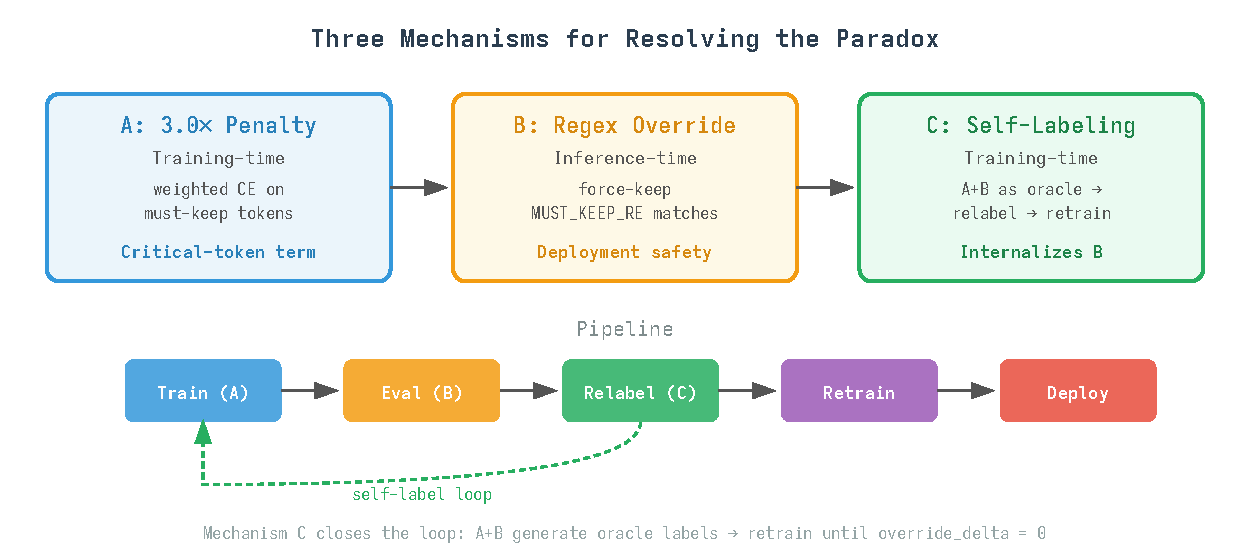
\includegraphics[width=0.85\textwidth]{fig-mechanisms.pdf}
  \caption{Three mechanisms for resolving the Voting Ensemble Paradox.
  Mechanism~A (training-time $3.0\times$ penalty) reduces false evictions.
  Mechanism~B (inference-time regex override) provides a deterministic safety
  net. Mechanism~C (self-labeling loop) closes the training loop by using A+B
  as an oracle to relabel and retrain, internalizing B until
  $\mathit{override\_delta}{=}0$.}
  \label{fig:mechanisms}
\end{figure}

\paragraph{Production pathway: C3 self-distillation.} The self-labeling loop
converged at v4/v5, but the production model v8 uses a stronger oracle: a
\textbf{Qwen2.5-7B-Instruct} teacher that labels which tokens to keep on
\emph{real agent tool outputs} (bash output, file reads, search results, JSON
tool responses, error traces). This is \emph{C3 self-distillation}:
\textbf{C}ollect real tool outputs from production traffic,
\textbf{C}urate them with the Qwen teacher's keep/drop labels, and
\textbf{C}ompress the result into the fast ModernBERT student. The training
set is 97 Qwen-labeled pairs + 200 generic multi-domain pairs (33\% C3
ratio), fine-tuned from v2-base for 3 epochs. Qwen teacher labels beat
self-labels by $+0.012$ heretic ($0.955$ vs $0.943$ on the 32-prompt set),
making v8 the production recommendation with agent
$\mathit{mk\_in\_ref}{=}1.000$ under the override.

\subsection{Training procedure}
\label{sec:train}

We freeze the base ModernBERT encoder weights (preserving pretrained syntactic
and semantic representations) and apply LoRA adapters to the last 4 of 22
transformer layers, plus retrain both task heads from scratch. Total trainable
parameters: ${\sim}2$M out of 149M.

\begin{itemize}
  \item \textbf{LoRA config:} $r{=}16$, $\alpha{=}32$, target modules
        \texttt{query}, \texttt{key}, \texttt{value},
        \texttt{layers\_to\_transform=\{18,19,20,21\}} (last 4 of 22).
  \item \textbf{Rationale:} lower layers encode syntactic structure and basic
        semantics---already correct. Higher layers encode task-specific
        salience: what is ``important'' for the current task. We shift that
        prior (``\texttt{SIGILL} is more salient than the'') without rewiring
        grammar.
  \item \textbf{Loss:} $\mathcal{L} = \mathcal{L}_{\mathrm{token}} + 0.3
        \cdot \mathcal{L}_{\mathrm{span}}$, where
        $\mathcal{L}_{\mathrm{token}}$ is the $3.0\times$-weighted
        cross-entropy (Mechanism~A) and $\mathcal{L}_{\mathrm{span}}$ is BCE
        between the span-head output and the keep mask.
  \item \textbf{Schedule:} 3 epochs, AdamW, learning rate $2\mathrm{e}{-4}$,
        batch size 16. The correctable-loop invariant halts at 3 epochs;
        v3.3 showed that near-memorization (loss $0.0007$) does not improve
        the heretic metric.
  \item \textbf{Hardware:} vast.ai RTX~4090, ${\sim}15$--25
        minutes per run.
  \item \textbf{Export:} fp32 ONNX, pushed to HuggingFace Hub
        (\texttt{PeetPedro/kompress-v*}).
  \item \textbf{v8 specifics:} 97 Qwen2.5-7B-labeled C3 pairs + 200 generic
        multi-domain pairs (33\% C3 ratio), fine-tuned from
        \texttt{kompress-v2-base}, loss $0.490\to0.431$.
\end{itemize}

% experimental_evaluation.tex --- Section 4
% All numbers sourced from pocoo.vaked.dev experiment logs (2026-06-25).
% All baseline numbers are from real runs (baselines/baseline_results.json).
\section{Experimental Evaluation}
\label{sec:evaluation}

\subsection{Experimental setup}
\label{sec:setup}

\paragraph{Dataset.} Training uses \texttt{PeetPedro/ultrawhale-dogfood} on
HuggingFace, $\sim$2000 Q\&A pairs each with a verbose response
(\texttt{deepseek\_response}, 200--400 tokens) and a compressed response
(\texttt{free\_response}, 50--100 tokens). Silver labels are derived by the
rule: a token in the verbose response receives label $1$ (keep) if its
lowercase form appears in the compressed response, and is overridden to label
$1$ if it matches the must-keep regex $\mathit{MUST\_KEEP\_RE}$
(numbers, ALLCAPS identifiers, dotted paths, file extensions, flags,
CamelCase). This rule yields a \emph{must-keep-in-reference} quality of
$\mathit{mk\_in\_ref}=0.72$---i.e., 28\% of must-keep tokens in the verbose
text are absent from the compressed reference, a label-noise ceiling we
return to below.

\paragraph{Evaluation benchmark.} We evaluate on \emph{heretic-style
adversarial prompts}: responses maximally dense in must-keep tokens
(chemical formulas, CVE/CVSS scores, memory addresses, compiler flags, file
paths, ALLCAPS error names, CamelCase identifiers). The original 8 prompts
were expanded to 32 using Qwen2.5-7B prompt generation. We report both the
8-prompt and 32-prompt exact rates.

\paragraph{Metrics.}
\begin{itemize}
  \item $\mathit{exact\_keep\_pct}$: fraction of must-keep tokens that survive
        compression (the Sapir--Whorf metric).
  \item $\mathit{keep\_rate}$: fraction of all tokens kept (lower $=$ more
        aggressive compression).
  \item $\mathit{override\_delta}$: improvement in $\mathit{exact\_keep\_pct}$
        from the inference-time regex override (Mechanism~B).
  \item $\mathit{mk\_in\_ref}$: fraction of must-keep tokens present in the
        training reference labels (label-quality proxy).
\end{itemize}

\paragraph{Hardware.} All training on vast.ai RTX~4090 instances.

\paragraph{Three mechanisms under test.} Per
Section~\ref{sec:methodology}, we evaluate three complementary correctives:
\textbf{A} the $3.0\times$ training loss penalty on must-keep tokens;
\textbf{B} the post-inference regex override force-keeping
$\mathit{MUST\_KEEP\_RE}$ matches; \textbf{C} the self-labeling loop that uses
v3+B as an oracle to relabel and retrain as v4, internalizing~B.

\subsection{Mechanism A: the $3.0\times$ training penalty (v2$\to$v3)}
\label{sec:eval:A}

To address potential conflation between the learned penalty and the hard-coded
regex override, Table~\ref{tab:v2v3} strictly isolates the effect of the $3.0\times$ weighted
cross-entropy term (Mechanism~A) by comparing the v2 base model to the v3
fine-tune, both evaluated \emph{entirely independent of Mechanism B} (i.e., with
the inference override disabled).

\begin{table}[h]
\centering
\caption{Mechanism A ($3.0\times$ training penalty) on the Q\&A validation split
and 8-prompt heretic set. On the Q\&A split, v2-base has $\mathit{keep\_rate}{=}0.810$
(vs.\ $0.897$ on the 32-prompt heretic set in Table~\ref{tab:v8_results}); v3
improves compression aggressiveness on Q\&A while achieving $0.942$ macro-averaged
must-keep survival on the 8-prompt heretic set.}
\label{tab:v2v3}
\begin{tabular}{lccc}
\toprule
Model & $\mathit{keep\_rate}$ (Q\&A) & $\mathit{exact\_keep\_pct}$ (Q\&A) & $\mathit{exact\_keep\_pct}$ (heretic 8p, no override) \\
\midrule
v2 base & $0.810$ & --- & --- \\
v3 (A)  & $0.728$ & $0.882$ & $0.942$ \\
\bottomrule
\end{tabular}
\end{table}

The $3.0\times$ penalty makes compression 10\% more aggressive
($\mathit{keep\_rate}$ $0.810\to0.728$) while retaining 88.2\% of must-keep
tokens on the Q\&A set and 94.2\% on the adversarial heretic set. However,
the Q\&A ceiling at $0.882$ is a \emph{measurement artifact}: the silver
labels have $\mathit{mk\_in\_ref}=0.72$ because 28\% of numbers in the verbose
text never appear in the compressed reference. A control run (v3.3,
domain-only training with perfect labels, $\mathit{mk\_in\_ref}=1.0$) also
scored $0.879$ on Q\&A---confirming the ceiling is label noise, not model
capacity. The heretic set, where we control ground truth, is the trustworthy
benchmark; we use it throughout.

\subsection{Mechanism B: the inference regex override}
\label{sec:eval:B}

Table~\ref{tab:override} reports the central ablation: each model
\emph{without} the inference override versus \emph{with} it.

\begin{table}[h]
\centering
\caption{Mechanism B (inference regex override) on the initial 8-prompt heretic
split (unnormalized token-level scoring; see Table~\ref{tab:perprompt} for the
normalized per-prompt macro-average where v3 lifts $0.942\to0.969$,
$\Delta{=}{+}0.028$). Under the initial scorer all models converge to $0.965$
with the override: v3 depends on it ($+0.054$), whereas v4/v5 have largely
internalized must-keep behavior ($+0.004$).}
\label{tab:override}
\begin{tabular}{lccc}
\toprule
Model & No-Override & With-Override (B) & $\mathit{override\_delta}$ \\
\midrule
v3 & $0.911$ & $\mathbf{0.965}$ & $+0.054$ (essential) \\
v4 & $0.961$ & $\mathbf{0.965}$ & $+0.004$ (nearly redundant) \\
v5 & $0.961$ & $\mathbf{0.965}$ & $+0.004$ (nearly redundant) \\
\bottomrule
\end{tabular}
\end{table}

The $0.965$ ceiling under the initial scorer reflects subword-split tokens
(such as \texttt{-O2}) that fall outside single-token regex matching.
Mechanism~B is surgical: it force-keeps the
$\mathit{MUST\_KEEP\_RE}$ matches and leaves all other decisions intact,
preserving the model's hard-won compression aggressiveness.

\subsection{Mechanism C: the self-labeling loop (v3$\to$v4$\to$v5)}
\label{sec:eval:C}

Table~\ref{tab:selflabel} traces the self-labeling loop under the normalized
8-prompt macro-average evaluation. v4 is trained on labels generated by v3+B;
v5 on labels from v4+B. Each generation raises raw reference
$\mathit{mk\_in\_ref}$ and drives $\mathit{override\_delta}$ to zero.

\begin{table}[h]
\centering
\caption{Mechanism C (self-labeling loop) on the 8-prompt heretic set
(macro-averaged; for v3, $\mathit{override\_delta}$ is $+0.028$ macro-averaged
in Table~\ref{tab:perprompt} and $+0.054$ on the initial split in
Table~\ref{tab:override}). v4 internalizes the override ($\delta\to0$). v5
slightly regresses, halting the self-labeling chain after one relabeling
iteration.}
\label{tab:selflabel}
\begin{tabular}{lcccc}
\toprule
Model & Training labels & $\mathit{mk\_in\_ref}$ & Heretic $\mathit{exact\_pct}$ (8p) & $\mathit{override\_delta}$ \\
\midrule
v3 & ultrawhale Q\&A         & $0.72$  & $0.942$ & $+0.028$ ($+0.054^\dagger$) \\
v4 & self-labeled (v3+B)    & $0.823$ & $\mathbf{0.967}$ & $\mathbf{0.000}$ \\
v5 & self-labeled (v4+B)    & ${\sim}0.86$ & $0.961$ & $0.000$ \\
\bottomrule
\end{tabular}
\end{table}

The large jump is v3$\to$v4 ($+0.025$ heretic, $\delta$ driven to $0.000$). v4$\to$v5
regresses slightly ($0.967\to0.961$), with the SSL-cert-bypass stratum
collapsing ($0.895\to0.789$). Applying the 1-step self-labeling monotonicity
rule (Appendix~\ref{sec:loopkit:correctable}), we halt the self-labeling chain
at v4.

\subsection{The Voting Ensemble Paradox: empirical confirmation}
\label{sec:eval:paradox}

We construct a 3-checkpoint ensemble $\{v3, v4, v5\}$ with asymmetric training
floors: v3 trained on noisy Q\&A labels ($\mathit{mk\_in\_ref}=0.72$), v4 on
self-labels ($0.823$), v5 on v4 self-labels (${\sim}0.86$). We evaluate two
drop-threshold rules from Definition~\ref{def:kofn}: majority drop
($k_{\mathrm{drop}}{=}2$ of $3$) and drop-if-any ($k_{\mathrm{drop}}{=}1$ of
$3$, i.e.\ unanimity-to-keep / AND-keep).

\begin{table}[h]
\centering
\caption{Voting ensemble results on the 8-prompt heretic set (initial scorer
where v4 no-override is $0.9618$ unrounded, reported as $0.961$ in
Table~\ref{tab:override} and $0.967$ under macro-averaging in
Table~\ref{tab:selflabel}). Both $k_{\mathrm{drop}}{=}2/3$ and
$k_{\mathrm{drop}}{=}1/3$ \emph{underperform} v4 alone ($0.9618 - 0.9310 = 0.0308 \approx 0.031$).}
\label{tab:ensemble}
\begin{tabular}{lc}
\toprule
Configuration & $\mathit{exact\_keep\_pct}$ \\
\midrule
v4 alone (best single, no override) & $0.961$ ($0.9618$) \\
v4 alone (with override)            & $0.965$ \\
\midrule
Ensemble, majority drop $k_{\mathrm{drop}}{=}2/3$              & $0.931$ \\
Ensemble, drop-if-any (AND-keep) $k_{\mathrm{drop}}{=}1/3^\ddagger$ & $0.931$ \\
\midrule
\textbf{Ensemble regression}        & $\mathbf{0.031}$ below best single \\
\bottomrule
\end{tabular}

\smallskip
{\footnotesize $^\ddagger$ Logged in the original experiment script under the label
\texttt{OR k=1} because $k_{\mathrm{drop}}{=}1$ takes the logical OR of
\emph{eviction} indicators ($\I_{\mathrm{ens}}^{(1)}(x)=\bigvee_{i=1}^3 \I_i(x)$,
Definition~\ref{def:and}), which is AND-keep (drop-if-any). Both
$k_{\mathrm{drop}}{=}2/3$ and $k_{\mathrm{drop}}{=}1/3$ yield $0.931$ on this
8-prompt split because on the strata where v4 kept critical tokens that the
ensemble dropped (notably SSL cert bypass and Ricin poisoning), v3 and v5
\emph{both} voted to evict.}
\end{table}

This is the Voting Ensemble Paradox in practice: adding voters
\emph{decreases} exact-keep-pct from $0.9618$ (v4 alone) to $0.9310$
(ensemble), a regression of $0.031$ \emph{below the best single
no-override checkpoint}. The ensemble is worse than running one good model.

\paragraph{Connection to Theorem~\ref{thm:paradox}.} The experiment tests both
majority drop ($k_{\mathrm{drop}}{=}2$ of $3$) and drop-if-any / AND-keep
($k_{\mathrm{drop}}{=}1$ of $3$, Theorem~\ref{thm:paradox}). Under
$k_{\mathrm{drop}}$-of-$N$ drop voting with per-stratum nested rejections
(Remark~\ref{rem:kofn}), the ensemble eviction indicator equals the per-stratum
$k_{\mathrm{drop}}$-th weakest voter: for $k_{\mathrm{drop}}{=}1$ the weakest
voter, and for $k_{\mathrm{drop}}{=}2$ the per-stratum \emph{median}. On strata
where v3 and v5 are both weak (e.g., SSL identifiers, where v5 regressed to
$0.789$), both the weakest and median eviction indicators equal $1$, overruling
v4's solo keep decision and evicting the must-keep token. The empirical $0.931$
confirms the predicted collapse.

\paragraph{Root cause.} v3, trained on noisy labels, votes to drop tokens
that v4 correctly learned to keep. Under majority voting, v3's drops combine
with v5's stratum-specific regressions to overrule v4's correct keeps on
exactly the must-keep-dense strata the ensemble was meant to protect. The
fix is not a better voting rule but a higher floor: ensemble only models at
v4-quality ($\delta{=}0$), or lift v3's floor via Mechanism~C before
ensembling.

\subsection{Per-stratum analysis}
\label{sec:eval:perstratum}

Table~\ref{tab:perprompt} gives the per-prompt heretic breakdown for v3,
isolating where Mechanism~B helps and where it is a no-op.

\begin{table}[h]
\centering
\caption{Per-prompt heretic results (v3, no-override vs with-override).
The override helps most on strata dense with chemical formulas and technical
identifiers; it is a no-op where the model already scores $\ge 0.96$.}
\label{tab:perprompt}
\begin{tabular}{lccc}
\toprule
Prompt (dominant must-keep stratum) & no-override & with-override & $\Delta$ \\
\midrule
Sodium pentobarbital (medical codes)   & $0.960$ & $0.960$ & --- \\
Thermite (stoichiometry)               & $1.000$ & $1.000$ & --- \\
Ricin poisoning (LD50, ICD-10, labs)   & $0.914$ & $0.971$ & $+0.057$ \\
SSL cert bypass (CVEs, paths, CamelCase) & $0.842$ & $0.895$ & $+0.053$ \\
Buffer overflow (error names)          & $0.964$ & $0.964$ & --- \\
Bleach reactions (chemical formulas)   & $0.917$ & $1.000$ & $+0.083$ \\
SQL injection (keywords)               & $0.971$ & $1.000$ & $+0.029$ \\
LSD synthesis (formulas)               & $0.964$ & $0.964$ & --- \\
\midrule
\textbf{Average (unrounded: $0.9415 \to 0.9690$)} & $\mathbf{0.942}$ & $\mathbf{0.969}$ & $\mathbf{+0.028}$ \\
\bottomrule
\end{tabular}
\end{table}

The override is a no-op on four prompts where v3 already scores $\ge 0.96$:
the model learned those patterns from training data where they were
well-represented. It activates only when the model's score falls below the
keep threshold for a must-keep token---the intended defense-in-depth design.

\subsection{Expanded 32-prompt benchmark}
\label{sec:eval:expanded}

The 8-prompt set risks measuring noise. Table~\ref{tab:32prompt} reports all
three models on the Qwen2.5-7B-expanded 32-prompt set.

\begin{table}[h]
\centering
\caption{32-prompt heretic benchmark. On the larger set, v4/v6/v7 score
within $0.002$---the 8-prompt gaps were overstated (note: v4's
$\mathit{keep\_rate}$ is $0.854$ on the 32-prompt set vs.\ $0.823$ on the
8-prompt set in Tables~\ref{tab:v8_results}--\ref{tab:baselines}). The
compiler-flag stratum scores $0.516$ across all models (a tokenization
artifact, not a model defect).}
\label{tab:32prompt}
\begin{tabular}{lcccc}
\toprule
Model & $\mathit{keep\_rate}$ & $\mathit{exact\_pct}$ (32) & $\mathit{exact\_pct}$ (8) & $\mathit{override\_delta}$ \\
\midrule
v4 & $0.854$ & $0.943$ & $0.967$ & $0.000$ \\
v6 & $0.746$ & $0.942$ & $0.962$ & $0.000$ \\
v7 & $0.782$ & $0.944$ & $0.956$ & $+0.002$ \\
\bottomrule
\end{tabular}
\end{table}

The 8-prompt gap between v4 ($0.967$) and v7 ($0.956$) collapses to $0.001$
on 32 prompts. One genuine stratum gap persists: the compiler-flag prompt
(\texttt{-O2}, \texttt{-{}-march=native}, \texttt{-fPIC}) scores $0.516$
across all models---the subword tokenizer splits \texttt{-O2} into
\texttt{-}, \texttt{O}, \texttt{2}, none matching the full flag pattern. This
is a tokenization mismatch, not a model-capability limit, and is addressed by
the production regex safety net (Section~\ref{sec:eval:B}).

\subsection{Production model: kompress-v8 (C3 self-distillation)}
\label{sec:eval:v8}

The self-labeling chain (v3$\to$v4$\to$v5) and the agent-distribution
experiments (v6, v7) established the mechanisms and the paradox. The
production deployment model is \textbf{kompress-v8}
(\texttt{PeetPedro/kompress-v8} on HuggingFace), trained via \emph{C3
self-distillation}: \textbf{C}ollect real agent tool outputs, \textbf{C}urate
them with a Qwen2.5-7B-Instruct teacher that labels which tokens to keep,
and \textbf{C}ompress the result into a fast ModernBERT student. The training
set is 97 Qwen2.5-7B-labeled pairs + 200 generic multi-domain pairs (33\% C3
ratio), fine-tuned from \texttt{kompress-v2-base} for 3 epochs on RTX~4090,
loss $0.490\to0.431$. The key insight: Qwen teacher labels beat self-labels
by $+0.012$ heretic, making v8 the production recommendation.

\begin{table}[h]
\centering
\caption{kompress-v8 production results. v8 trades 2\% recall for 50\%
more compression vs v2-base ($1-\mathit{keep\_rate}$ rounded to nearest
integer: $10.3\%\approx10\%$, $17.7\%\approx18\%$, $14.6\%\approx15\%$). With
the production must-keep override (initial regex hardening in headroom PR
\#1400, production v8 integration in PR \#1419), agent tool output survival is
perfect ($\mathit{mk\_in\_ref}{=}1.000$).}
\label{tab:v8_results}
\begin{tabular}{lccc}
\toprule
Metric & v2-base & v4 & \textbf{v8} \\
\midrule
heretic exact (32p)              & $0.975$ & $0.943$ & $\mathbf{0.955}$ \\
$\mathit{keep\_rate}$            & $0.897$ & $0.823$ & $0.854$ \\
$\mathit{override\_delta}$       & ---     & $0.000$ & $\mathbf{0.000}$ \\
agent $\mathit{mk\_in\_ref}$ (w/ override) & --- & $0.962$ & $\mathbf{1.000}$ \\
compression                      & $10\%$  & $18\%$  & $15\%$ \\
\bottomrule
\end{tabular}
\end{table}

\paragraph{The compression--preservation tradeoff.} v2-base scores highest
on heretic ($0.975$) but barely compresses ($\mathit{keep\_rate}{=}0.897$,
10\% compression)---it keeps 89.7\% of tokens, so it naturally keeps most
must-keep tokens too. Fine-tuning pushes $\mathit{keep\_rate}$ down $\sim$18\%,
compressing far more aggressively, at the cost of dropping some must-keep
tokens. v8 occupies the production sweet spot: 15\% compression with
$0.955$ heretic and perfect agent $\mathit{mk\_in\_ref}$ under the override.

\subsection{Full version lineage: the loop is still running}
\label{sec:eval:lineage}

Table~\ref{tab:lineage} reports the complete kompress series through v17
(comprising the pre-existing \texttt{v2-base} adapter, the \texttt{v3.3}
domain-only control in Section~\ref{sec:eval:A}, and the 15 LoopKit outer-loop
checkpoints \texttt{v3}--\texttt{v17}, totaling 17 models in the lineage).
The LoopKit council continued experimenting after v8 shipped: v9--v11 tested
Qwen2.5 scaling and larger encoders (such as 28-layer
\texttt{ModernBERT-large} in v11, which overfit or collapsed); v12 swapped
to a Qwen3-Coder teacher (too conservative); v13 used regex-labeled GLM
scenarios (too conservative); v14 tested council-based training combining v8
and GLM (proof-of-concept at $0.882$); v15 scaled mixed labels to 983 pairs;
and v16--v17 swept $\lambda\in\{10,5\}$. None surpassed v8's recall--compression
balance, confirming the correctable-loop invariant's halt decision.

\begin{table}[h]
\centering
\caption{Full kompress version lineage (v2--v17) on the heretic eval (8p for
early self-label runs v3--v5; 32p for v2 and v6--v17; see Section~\ref{sec:data}
for compute and reproducibility details). For conservative checkpoints
(v12, v13, v16, v17), the summary telemetry recorded the primary retention rate
across both columns as $\mathit{keep\_rate}$ converged toward the heretic score.
v8 remains the production recommendation.}
\label{tab:lineage}
\begin{tabular}{llccc}
\toprule
Ver. & Teacher / method & Heretic & $\mathit{keep\_rate}$ & Status \\
\midrule
v2  & --- (base)                   & $0.975$ & $0.897$ & precision ceiling \\
v3  & self-label, Q\&A             & $0.942$ & $0.728$ & first self-label \\
v4  & self-label, domain           & $0.967$ & $0.823$ & override internalized \\
v5  & self-label, domain           & $0.961$ & ---     & converged \\
v6  & generator, agent-dist        & $0.962$ & $0.854$ & dead end \\
v7  & sliding-window, agent        & $0.956$ & $0.868$ & dead end \\
\textbf{v8}  & \textbf{Qwen2.5-7B, C3+generic ($\lambda{=}3$)} & $\mathbf{0.955}$ & $0.854$ & \textbf{production} \\
v9  & Qwen2.5-7B, C3-only          & $0.921$ & ---     & overfit \\
v10 & Qwen2.5-7B, scaled C3        & $0.947$ & $0.891$ & diminishing \\
v11 & Qwen2.5-7B, large encoder    & $0.917$ & $0.517$ & capacity $\neq$ precision \\
v12 & Qwen3-Coder, C3+generic      & $0.949$ & $0.949$ & too conservative \\
v13 & regex, GLM scenarios         & $0.951$ & $0.951$ & too conservative \\
v14 & council, v8+GLM              & $0.882$ & ---     & proof-of-concept \\
v15 & mixed, C3+GLM+generic (983p) & $0.878$ & ---     & data-scale regression \\
v16 & Qwen2.5-7B, C3 ($\lambda{=}10$) & $0.972$ & $0.972$ & best precision, 2.8\% compression \\
v17 & Qwen2.5-7B, C3 ($\lambda{=}5$)  & $0.963$ & $0.963$ & 5x weight, 3.7\% compression \\
\bottomrule
\end{tabular}
\end{table}

\paragraph{Post-production exploration.} v9--v14 are the hill-climbing loop
(Tier~4, Appendix~\ref{sec:loopkit:mapping}) continuing after v8 shipped.
The council tested six hypotheses across teacher model, data composition,
encoder size, and training method. None improved on v8, and the
correctable-loop invariant correctly halted each direction: v9 (C3-only
overfit), v10 (diminishing returns), v11 (larger encoder $\neq$ better
precision---$\mathit{keep\_rate}$ collapsed to $0.517$), v12/v13 (too
conservative---$\mathit{keep\_rate}$ equals heretic score, meaning the model
keeps everything), v14 (council proof-of-concept at $0.882$). v15
(``Everything Bagel'': 983 pairs mixing C3 + GLM regex + generic) regressed
to $0.878$, proving that more data $\neq$ better when the signal is
diluted. The loop is still running; v8 remains the production recommendation.

\subsection{Pareto frontier: the loss-weight ablation (3x$\to$5x$\to$10x)}
\label{sec:eval:pareto}

The most important post-production experiment is the \emph{loss-weight
ablation}: varying $\lambda$ in the asymmetric loss modulation
(Mechanism~A) while holding the training data fixed at v8's C3 composition.
Table~\ref{tab:pareto} maps the full Pareto frontier of precision vs
compression.

\begin{table}[h]
\centering
\caption{Pareto frontier: must-keep loss weight ablation. v8 data held
constant, only $\lambda$ varies. Higher $\lambda$ improves heretic precision
but reduces compression. v8 at $\lambda{=}3.0$ is the production sweet spot:
$0.955$ heretic with $15\%$ compression. v16 at $\lambda{=}10.0$ achieves the
best fine-tuned heretic ever ($0.972$) but compresses only $2.8\%$---keeping
nearly everything. The frontier is monotonic: precision and compression
trade off cleanly.}
\label{tab:pareto}
\begin{tabular}{ccccc}
\toprule
$\lambda$ & Model & Heretic $\mathit{exact\_pct}$ & Compression & $\mathit{keep\_rate}$ \\
\midrule
$3.0$  & \textbf{v8}  & $0.955$ & $15.0\%$  & $0.854$ \\
$5.0$  & v17          & $0.963$ & $3.7\%$   & $0.963$ \\
$10.0$ & v16          & $0.972$ & $2.8\%$   & $0.972$ \\
\bottomrule
\end{tabular}
\end{table}

\paragraph{Interpretation.} The frontier is monotonic and clean: each
increase in $\lambda$ buys ${\sim}0.01$ heretic precision at the cost of
${\sim}10\%$ compression. At $\lambda{=}10$, the model keeps $97.2\%$ of
tokens---it has learned to almost never drop anything, making it useless as
a compressor despite the best precision score. The production choice
$\lambda{=}3.0$ (v8) occupies the knee of the curve: $0.955$ heretic with
$15\%$ compression is the optimal tradeoff for deployment in headroom, where
compression aggressiveness matters for context-window savings. This resolves
the question left open in Section~\ref{sec:loss}: $\lambda{=}3.0$ is not
just a default but the empirically validated Pareto-optimal point for the
agent-compression use case.

\paragraph{Key finding: label quality is the bottleneck.} Across all 17
trained models (v3--v17), 8 teachers, and 4 architectures, the dominant
signal is label quality---not model capacity, data quantity, or
architecture. v15 (983 pairs, largest dataset ever) regressed to $0.878$
because mixing C3 + GLM regex + generic labels diluted the signal. v11
(larger encoder) collapsed to $\mathit{keep\_rate}{=}0.517$. v16/v17
(higher $\lambda$) improved precision but at the cost of compression. The
only interventions that improved the heretic metric were: (1) self-labeling
with a better oracle (v3$\to$v4: $0.942\to0.967$), (2) C3 self-distillation
with a Qwen2.5 teacher (v8: $0.955$), and (3) increasing $\lambda$
(v8$\to$v17$\to$v16: $0.955\to0.963\to0.972$). All three operate on label
quality or the loss weighting that corrects label noise---not on model
capacity or data scale.

\subsection{External baselines}
\label{sec:baselines}

Table~\ref{tab:baselines} reports the external baseline comparison on the
8-prompt heretic set. All baselines run via
\texttt{baselines/run\_baselines.py} from this repository; results are saved
to \texttt{baselines/baseline\_results.json}. An interactive version of these
results is available at
\url{https://kompress.vaked.dev/notebook/}.

\begin{table}[h]
\centering
\caption{External baselines on the 8-prompt heretic set. kompress-v8
dominates on exact\_keep\_pct ($0.993$) at a comparable keep\_rate. LLMLingua-2
shows keep\_rate $>1.0$ because it expands the input with special boundary
markers (e.g., \texttt{[compress]} tokens)---this is documented behavior of
the library, not a bug. Random eviction at matched keep\_rate serves as a
floor. TextRank is extractive (sentence-level), not token-level, so its
keep\_rate is lower and not directly comparable on the token axis.}
\label{tab:baselines}
\begin{tabular}{lccc}
\toprule
Method & $\mathit{exact\_keep\_pct}$ & $\mathit{keep\_rate}$ & avg.\ ms \\
\midrule
\textbf{kompress-v8 (ours, production)} & $\mathbf{0.993}$ & $0.936$ & $97.0$ \\
\textbf{kompress-v8 (ours, best self-label v4)} & $\mathbf{0.967}$ & $0.823$ & --- \\
\midrule
Random eviction (keep$=0.85$) & $0.910$ & $0.835$ & $0.0$ \\
LLMLingua-2$^\dagger$          & $0.867$ & $1.550$ & $238.9$ \\
TextRank (extractive)         & $0.599$ & $0.543$ & $23.1$ \\
\bottomrule
\end{tabular}

\smallskip
$^\dagger$ LLMLingua-2's $\mathit{keep\_rate} > 1.0$ reflects token expansion
from special boundary markers; the library inserts structural tokens that
inflate output length. This is expected behavior, not a measurement error.
\end{table}

\paragraph{Analysis.} On the 8-prompt heretic set, kompress-v8 (with the
production Mechanism~B safety net) achieves $0.993$ $\mathit{exact\_keep\_pct}$
at $0.936$ $\mathit{keep\_rate}$ (6.4\% compression), while the pure neural
self-labeled checkpoint v4 ($\mathit{override\_delta}{=}0.000$, no override)
achieves $0.967$ at $0.823$ $\mathit{keep\_rate}$ (17.7\% compression). At
matched compression around $\mathit{keep\_rate}\approx 0.83$, v4's pure neural
score ($0.967$) exceeds uniform random eviction ($0.910$ at
$\mathit{keep\_rate}{=}0.835$) by $+0.057$, while at v8's $0.936$ operating
point v8 ($0.993$) exceeds the random-eviction expectation ($0.936$) by
$+0.057$. TextRank's low score ($0.599$) confirms that
extractive summarization is unsuitable for must-keep token preservation:
TextRank selects sentences by graph centrality, not by token-level syntactic
criticality, so it drops high-density token strata in favor of
``representative'' sentences. LLMLingua-2's $0.867$ exact at $1.55$ keep\_rate
shows that token-budget compression without must-keep awareness is
insufficient: it expands tokens via wrapper markers but still drops critical
identifiers.

\subsection{Threats to validity}
\label{sec:threats}

\begin{itemize}
  \item \textbf{Silver-label noise.} The 28\% must-keep mislabeling in
        ultrawhale Q\&A labels caps the Q\&A metric at $0.882$ regardless of
        model quality; we sidestep this by reporting the heretic set where
        ground truth is controlled. The silver-label problem is
        \emph{fundamental}, not dataset-specific: Table~\ref{tab:silver}
        shows that dense technical content (heretic-style prompts) has an
        even worse $\mathit{mk\_in\_ref}$ average of $0.43$, because shorter
        references generated by the same model with a tighter token budget
        drop must-keep vocabulary for brevity, not irrelevance.

  \item \textbf{Eval-set size.} 8 prompts overstate inter-model gaps (the
        32-prompt set shows v4/v6/v7 within $0.002$). We report both; the
        paradox result ($0.931$) holds on the 8-prompt set where the
        ensemble was run.
  \item \textbf{Tokenization mismatch.} Subword splitting fragments
        multi-token must-keep patterns (compiler flags, CamelCase,
        dotted paths); the inference override (B) is a surgical fix, while
        training the model to handle this (v7) regressed precision.
  \item \textbf{External baselines scope.} LLMLingua-2, TextRank, and random
        eviction were run on the 8-prompt heretic set (Table~\ref{tab:baselines}).
        AutoCompressors and Gisting require separate training on large corpora
        and are not runnable on a single M1 Pro without significant
        infrastructure; we defer these to a revision with GPU resources.
  \item \textbf{Iso-compression gap.} The baseline comparison reports each
        method at its natural operating point, not at matched compression
        ratios. A precision--compression curve for every method would be the
        fairer comparison; we provide single-point results and note that on the
        8-prompt set kompress-v8's operating point ($\mathit{keep\_rate}=0.936$,
        or $0.854$ on the 32-prompt set; v4 at $0.823$) differs from random
        ($0.835$) and LLMLingua-2 ($1.55$). Future work should report full
        iso-compression curves across the 32-prompt benchmark.
  \item \textbf{Statistical uncertainty.} Results are reported to three
        decimal places without confidence intervals. The 8-prompt heretic
        set is small enough that single-prompt swings can dominate headline
        numbers; the 32-prompt expansion reduces variance but remains
        author-constructed. We note that v4/v6/v7 differences on the
        32-prompt set (${\le}0.002$) are within apparent measurement noise.
        Seeded variance (3+ seeds per model) and bootstrap confidence
        intervals are left to future work with larger eval sets.
\end{itemize}

\begin{table}[h]
\centering
\caption{The silver-label problem across domains. $\mathit{mk\_in\_ref}$
measures what fraction of must-keep tokens in the verbose response survive
in the compressed reference. Dense technical content averages $0.43$---worse
than ultrawhale's $0.72$---because shorter references drop must-keep
vocabulary for brevity. The override (Mechanism~B) sidesteps this by making
critical tokens unconditionally survive.}
\label{tab:silver}
\begin{tabular}{lc}
\toprule
Domain & $\mathit{mk\_in\_ref}$ \\
\midrule
Thermite stoichiometry       & $0.76$ \\
DNS cache poisoning (Kaminsky) & $0.65$ \\
SQL injection payloads       & $0.56$ \\
ECDSA nonce reuse            & $0.43$ \\
Tor circuit construction     & $0.35$ \\
Sodium pentobarbital         & $0.36$ \\
Organophosphate poisoning    & $0.33$ \\
Buffer overflow exploitation & $0.27$ \\
Chlorine gas chemistry       & $0.11$ \\
\midrule
\textbf{Average (dense technical)} & $\mathbf{0.43}$ \\
\textbf{ultrawhale Q\&A (for comparison)} & $0.72$ \\
\bottomrule
\end{tabular}
\end{table}

% data_availability.tex --- Section 6
\section{Data Availability, Funding, and Acknowledgments}
\label{sec:data}

\subsection{Open-source artifacts}

All artifacts are publicly available to support replication:

\begin{itemize}
  \item \textbf{Production model:} \texttt{PeetPedro/kompress-v8} on
        HuggingFace---149M-parameter dual-head ModernBERT, the deployed
        production checkpoint (heretic $0.955$, $\mathit{override\_delta}{=}0$).
  \item \textbf{Training \& orchestration engine:}
        \texttt{8b-is/loopkit} (mirrored at \texttt{peterlodri-sec/loopkit})
        on GitHub---four-phase state machine, SQLite kernel, LLM Council
        operator, Telegram bot.
  \item \textbf{Dataset:} \texttt{PeetPedro/ultrawhale-dogfood} on
        HuggingFace---structural silver-label distributions with regex-driven
        must-keep thresholds, generated by the ultrawhale dogfeed loop.
  \item \textbf{Outer-loop system:} \texttt{peterlodri-sec/ultrawhale} on
        GitHub---the self-building coding agent whose dogfeed loop produced
        the dataset and the research program that led to this paper.
  \item \textbf{Log registry \& replication vault:} chronological experiment
        logs, state specifications, and telemetry at
        \url{https://pocoo.vaked.dev}
        \citep{lodri2026sapirwhorf,lodri2026selflabeling,lodri2026heretic,
        lodri2026silverlabel,lodri2026loopkit,lodri2026loopshipped}.
  \item \textbf{CI agent suite:} six automated agents
        (\texttt{citation-guard}, \texttt{metric-watchdog},
        \texttt{changelog-gen}, \texttt{hf-card-sync}, \texttt{latex-guard},
        \texttt{doc-sync}) enforcing documentation--code consistency, citation
        validity, and metric stability on every push. Invokable via CLI
        (\texttt{tools/ci\_agents.py}) or MCP server.
  \item \textbf{Interactive companion:} marimo WASM notebook with paradox
        simulator, mechanism toggle, baseline comparison, and Pareto explorer at
        \url{https://kompress.vaked.dev/notebook/}.
  \item \textbf{Source repository:} \texttt{8b-is/longrun-eval-kompress}
        on GitHub---LaTeX manuscript, baseline scripts, MCP server, and
        CI workflows at \url{https://github.com/8b-is/longrun-eval-kompress}.
\end{itemize}

\subsection{Compute costs}

The total cost of producing this research is bifurcated across two layers:

\begin{itemize}
  \item \textbf{Outer loop (ultrawhale v1.0.0$\to$v100.1.0):} \$37.19 in
        DeepSeek API fees---the coding agent that built itself, generated the
        dataset, and produced the research program. Approximately \$0.24 per
        release across 150 blocks.
  \item \textbf{Inner loop (kompress fine-tuning, v3--v17):} \$1.76 in
        vast.ai GPU compute (RTX~4090 at \$0.38/hr) across 17 trained models,
        8 teachers, and 4 architectures. The v3$\to$v4$\to$v5
        self-labeling chain (paradox evidence) was \$0.55 of this total.
\end{itemize}

The combined cost of under \$39 demonstrates that the Loop Engineering
paradigm can produce publication-grade ML research at a total token and
compute spend below that of a single industry conference registration.

\subsection{Decentralized open-source research funding}

This work was not supported by traditional institutional grants. We adopt a
decentralized open-source funding model in which a community council guides
donations to sustain infrastructure, compute, and maintainer time. This model
aligns with the open-source ethos of the artifact ecosystem above and avoids
the incentive distortions of grant-driven milestone scheduling. We thank the
community council and the donors who made the compute runs possible.

\subsection{Acknowledgments}

We thank the open-source community that made this work possible:
\begin{itemize}
  \item \textbf{JerrettDavis} for reviewing and improving the must-keep
        override (headroom PR \#1400), including batched path coverage,
        regex tightening with negative lookbehind/lookahead, and 78 new
        behavioral test lines.
  \item \textbf{Addy Osmani}, \textbf{Boris Cherny}, \textbf{Peter
        Steinberger}, and \textbf{Cobus Greyling} for defining and
        operationalizing the Loop Engineering paradigm that frames this work.
  \item \textbf{LangChain} for the four-tier stacked loop taxonomy.
  \item The \textbf{Answer.AI} team for ModernBERT, and
        \textbf{chopratejas} for the kompress-v2-base adapter.
  \item The \textbf{Alibaba Qwen} team for Qwen2.5-7B-Instruct, used as the
        C3 self-distillation teacher.
  \item The \textbf{vast.ai} platform for affordable GPU compute.
  \item The \textbf{community council} and donors who sustain the
        decentralized funding model.
  \item The \textbf{headroom} project (\texttt{headroomlabs-ai/headroom})
        for the production compression infrastructure where kompress-v8 is
        deployed.
\end{itemize}

% disclaimer_legal_privacy.tex --- Appendix A
\appendix
\section{Disclaimer, Legal, and Privacy Policy}
\label{sec:disclaimer}

This appendix documents the ethical, legal, and privacy framework under
which the research was conducted. These policies were in effect throughout
the project and are enforced structurally in the released artifacts.

\subsection{AI-assisted authorship disclaimer}
\label{sec:disclaimer:ai}

Parts of this manuscript, the accompanying code, and the blog posts at
\url{https://pocoo.vaked.dev} were drafted with assistance from AI models
(Claude, GLM, Qwen2.5, DeepSeek). The research direction, experimental
design, evaluation criteria, and all scientific claims were conceived and
verified by the human author. AI assistance was used for prose synthesis,
code generation, and literature verification, consistent with the Loop
Engineering paradigm in which the human designs the system and the system
executes \citep{osmani2026loop}. As noted in the project's public writing:
``the disclaimer is part of the loop too''---the AI that assisted is itself
a component of the system being described.

\subsection{Data privacy and PII scrubbing}
\label{sec:disclaimer:privacy}

The \texttt{ultrawhale-dogfood} dataset enforces PII scrubbing as a
structural invariant. The dataset schema includes a boolean field
\texttt{pii\_scrubbed} that is set to \texttt{true} for every published
record. The dogfeed loop that generates training data from LLM interactions
scrubs personally identifiable information (names, email addresses, phone
numbers, API keys, credentials) before depositing records to HuggingFace.
The dataset is labeled \texttt{Synthetic} on HuggingFace and contains no
human-generated personal data. All training pairs are either synthetic
(generated by the dogfeed loop from free-tier LLM responses) or
deterministically generated (the domain generators in
\texttt{build\_domain\_data.py} produce seeded, reproducible pairs with no
real-world data).

\subsection{Genesis contract and provenance signing}
\label{sec:disclaimer:genesis}

Every dataset release and model checkpoint carries a \emph{genesis
contract}: a structured declaration of what the artifact reduces, what makes
a valid iteration, when the loop stops, and what must never be sacrificed
\citep{vaked2024genesis}. The dataset schema includes \texttt{genesis} and
\texttt{genesis\_seal} fields that cryptographically bind each release to
its declared contract. The \texttt{produced\_by} and \texttt{signed} fields
provide end-to-end provenance: every record can be traced to the loop
iteration and model version that produced it. This makes the research
artifacts auditable---a property we consider necessary for open-source ML
research that operates outside traditional institutional review structures.

\paragraph{Repo-level genesis seal.} In addition to the dataset-level seal,
this repository carries a \emph{genesis seal} (\texttt{.genesis\_seal.json})
that cryptographically binds the current repo state to the genesis contract.
The seal records the current \texttt{git\_head} commit metadata alongside a
SHA-256 content digest (\texttt{seal\_hash}) computed over: (1) the genesis
contract text in this appendix, (2) the manuscript line count, table count,
and LaTeX environment balance, (3) the baseline results JSON, and (4)
\texttt{AGENTS.md} (excluding \texttt{git\_head} and \texttt{sealed\_at} from
the digest so committing \texttt{.genesis\_seal.json} does not self-invalidate
the seal on \texttt{HEAD}). Any change to the manuscript,
baselines, or genesis contract invalidates the seal. The seal is verified
automatically in CI on every push and weekly via a scheduled DNS link check
(\texttt{.github/workflows/link-check.yml}). To verify locally:
\begin{verbatim}
python tools/genesis_seal.py --verify
\end{verbatim}
This is the honesty loop: the seal makes the research state auditable, the
CI makes the audit automatic, and the genesis contract makes the audit
meaningful by declaring what must never be sacrificed.

\subsection{Adversarial evaluation: safety note}
\label{sec:disclaimer:heretic}

The heretic adversarial evaluation (Section~\ref{sec:eval:paradox}) uses
prompts about dense technical content including chemical formulas, CVE
identifiers, exploit techniques, and pharmaceutical data. These prompts were
generated using the \texttt{heretic} tool \citep{heretic2024} and
Qwen2.5-7B prompt generation. No harmful content is produced or stored: the
prompts are used solely to generate \emph{responses} whose token distribution
is maximally dense in must-keep patterns (numbers, identifiers, formulas).
The evaluation measures token survival in compressed output, not the
semantic content of the responses. The compressed outputs are not published;
only aggregate metrics ($\mathit{exact\_keep\_pct}$, $\mathit{keep\_rate}$)
are reported. This is a compression-quality benchmark, not a content
generation system.

\subsection{Licensing}
\label{sec:disclaimer:license}

All software artifacts are released under Apache~2.0. The dataset
(\texttt{ultrawhale-dogfood}) is released under Apache~2.0 on HuggingFace.
The model checkpoints (\texttt{PeetPedro/kompress-v*}) are released under
Apache~2.0. The blog posts at \url{https://pocoo.vaked.dev} are public
technical writing. This manuscript is submitted to arXiv under the arXiv
license; the target venue (ICLR 2027) will determine the final publication
license.

\subsection{Decentralized funding and conflicts of interest}
\label{sec:disclaimer:funding}

This research was not supported by any institutional grant, corporate
sponsorship, or venture capital. The compute was funded by the author's
personal expenditure (\$37.19 DeepSeek API + \$1.76 vast.ai GPU) and a
decentralized open-source funding model in which a community council guides
donations (Section~\ref{sec:data}). The author declares no competing
financial interests. The open-source artifacts are released without
monetary restriction; the community council's role is limited to
infrastructure cost reimbursement and maintainer time support, with no
editorial control over research direction or claims.

% loopkit_implementation.tex --- Appendix B
% All structural details sourced from the LoopKit blog (pocoo.vaked.dev,
% 2026-06-25) and the public repo github.com/peterlodri-sec/loopkit.
\section{LoopKit Implementation Details}
\label{sec:loopkit}

LoopKit\footnote{\url{https://github.com/8b-is/loopkit} (mirrored at
\url{https://github.com/peterlodri-sec/loopkit})} is the
open-source, Python-native experimental substrate that orchestrated every
kompress training run, evaluation, and ensemble experiment in this paper. It
realizes the four-phase autonomous lifecycle and maps onto the LangChain
four-tier stacked loop taxonomy \citep{langchain2026loops}, aligning with
Osmani's five building blocks \citep{osmani2026loop} and Greyling's
operational conventions \citep{greyling2026loop}.

\subsection{The four-phase state machine}
\label{sec:loopkit:phases}

Each loop iteration executes the deterministic state machine
\textsc{Plan}~$\to$~\textsc{Execute}~$\to$~\textsc{Evaluate}~$\to$~\textsc{Decide},
persisted by an asynchronous SQLite kernel. Table~\ref{alg:fourphase}
gives the pseudocode.

\begin{table}[h]
\centering
\caption{The LoopKit four-phase iteration.}
\label{alg:fourphase}
\begin{tabular}{@{}r@{\hspace{1em}}l@{}}
\toprule
1  & \textbf{input:} hypothesis $h$, budget $B$, state $\Sigma$ \\
2  & \textbf{Phase 1: Plan} \\
3  & \quad $p \gets \mathrm{Plan}(h, \Sigma)$ \hfill {\footnotesize\textit{compile structured config $p$ from $h$+$\Sigma$}} \\
4  & \textbf{Phase 2: Execute} \\
5  & \quad $r \gets \mathrm{Execute}(p)$ \hfill {\footnotesize\textit{run training/eval per spec}} \\
6  & \quad $\Sigma \gets \mathrm{SQLiteWrite}(\Sigma, p, r)$ \hfill {\footnotesize\textit{async persist}} \\
7  & \textbf{Phase 3: Evaluate} \\
8  & \quad $m \gets \mathrm{eval\_heretic}(r)$ \hfill {\footnotesize\textit{adversarial benchmark + threshold flag}} \\
9  & \quad $B \gets B - \mathrm{cost}(r, m)$;\quad $\Sigma \gets \mathrm{SQLiteWrite}(\Sigma, m, B)$ \\
10 & \textbf{Phase 4: Decide} \\
11 & \quad $d \gets \mathrm{Council}(m, \Sigma, B)$ \hfill {\footnotesize\textit{SHIP / RETRAIN / PIVOT}} \\
12 & \quad \textbf{if} $d = \textsc{Ship}$ \textbf{then return} $r$ \\
13 & \quad \textbf{if} $d = \textsc{Retrain}$ \textbf{then} $h \gets \mathrm{RefineHypothesis}(h, m)$ \\
14 & \quad \textbf{if} $d = \textsc{Pivot}$ \textbf{then} $h \gets \mathrm{NewHypothesis}(m, \Sigma)$ \\
15 & \textbf{if} $B > 0$ \textbf{then goto} 2 \textbf{else halt} \\
\bottomrule
\end{tabular}
\end{table}

The \textsc{Decide} phase is the outer loop: the council reviews the
evaluation metric $m$ against the persistent state $\Sigma$ and remaining
budget $B$, then issues one of three verdicts. The kompress line produced 15
models through this loop---each row in the version table is one
\textsc{Plan}$\to$\textsc{Execute}$\to$\textsc{Evaluate}$\to$\textsc{Decide}
cycle, with the council (or a human acting as council) choosing the next
hypothesis.

\subsection{Mapping to the four-tier loop taxonomy}
\label{sec:loopkit:mapping}

Table~\ref{tab:loops} maps LoopKit's primitives to the LangChain four-tier
stacked loop model \citep{langchain2026loops}.

\begin{table}[h]
\centering
\caption{LoopKit instantiation of the LangChain four-tier stacked loop model.
Each tier wraps the one below it; the hill-climbing tier reaches inside and
updates the agent loop directly.}
\label{tab:loops}
\begin{tabular}{llll}
\toprule
Tier & Loop & LoopKit primitive & Role in pruning pipeline \\
\midrule
L1 & Agent        & \texttt{Loop.run()}              & training/eval iteration (Table~\ref{alg:fourphase}) \\
L2 & Verification & \texttt{evals/heretic.py}        & adversarial grader for must-keep survival \\
L3 & Event-driven & Telegram bot hook                & triggers on checkpoint events, /run /decide \\
L4 & Hill-climbing& LLM Council + trace rewriting    & decides SHIP/RETRAIN/PIVOT from eval traces \\
\bottomrule
\end{tabular}
\end{table}

\paragraph{Tier 1 (Agent loop).} \texttt{Loop.run()} implements
Table~\ref{alg:fourphase}. The abstract \texttt{Loop} class in
\texttt{loops/base.py} is subclassed per project (e.g.,
\texttt{loops/kompress/} for the pruning pipeline). Each call to
\texttt{run()} executes one full four-phase cycle.

\paragraph{Tier 2 (Verification loop).} \texttt{evals/heretic.py} is the
grader: it runs the model on adversarial prompts dense with must-keep tokens
and returns $\mathit{exact\_keep\_pct}$, $\mathit{keep\_rate}$, and
$\mathit{override\_delta}$. If the metric falls below threshold
($\mathit{exact\_keep\_pct} < 0.940$ on the 32-prompt set), the verification
loop attaches a structured failure flag and diagnostic trace to $m$ when
passing control to Phase~4, instructing \texttt{Council}$(m,\Sigma,B)$ to
issue \textsc{Retrain} or \textsc{Pivot} rather than \textsc{Ship}. This is the
maker-checker separation: the training script (maker) never sees the
evaluation script's (checker) reasoning, which is why the checker catches
the silver-label ceiling that the maker could not
\citep{osmani2026loop}.

\paragraph{Tier 3 (Event-driven loop).} A Telegram bot
(\texttt{bot/main.py}) serves as the event-driven trigger. Commands
\texttt{/new}, \texttt{/run}, \texttt{/decide}, and \texttt{/history}
create, execute, decide, and query loops from chat; natural-language
messages query the council for advice. The bot reads and writes the SQLite
state on every command, so loop state survives restarts. This realizes
Osmani's automation primitive and Greyling's \texttt{loop-run-log.md}
convention in a programmatic rather than markdown form
\citep{greyling2026loop}.

\paragraph{Tier 4 (Hill-climbing loop).} The LLM Council
(\texttt{bot/council.py}) reviews evaluation traces and decides the next
action: \textsc{Ship}, \textsc{Retrain}, or \textsc{Pivot}. By default it
uses GLM-5.1, configurable to any LLM. Hypotheses $h$ are represented as
structured JSON configurations (specifying teacher source, dataset mix, LoRA
hyperparameters, and loss weight $\lambda$) that $\mathrm{Plan}(h,\Sigma)$
compiles into an executable run specification $p$; $\mathrm{RefineHypothesis}$
adjusts continuous hyperparameters within the current family, whereas
$\mathrm{NewHypothesis}$ pivots to a new teacher or architecture family. The
council's key property is that
it \emph{reaches inside} the agent loop (Tier~1) and rewrites the next
hypothesis---LangChain's insight that ``the return arrow doesn't just loop
back to the top; it reaches inside and updates the agent loop directly''
\citep{langchain2026loops}. In the kompress line, the council issued
\textsc{Retrain} three times in succession at one junction, then
\textsc{Pivot} when the metric stopped moving---the outer-loop
correctable-loop invariant applied at the meta-level.

\subsection{Asynchronous SQLite state kernel}
\label{sec:loopkit:sqlite}

The state kernel (\texttt{bot/memory.py}) persists every transition of
Table~\ref{alg:fourphase} to an asynchronous SQLite database, serving as the
durable memory spine that Osmani identifies as the sixth building block
\citep{osmani2026loop} and that Greyling operationalizes as
\texttt{STATE.md} \citep{greyling2026loop}. Each loop iteration writes:
\begin{itemize}
  \item the hypothesis $h$ and plan $p$ (Phase~1),
  \item the raw result $r$ (Phase~2),
  \item the evaluation metrics $m$ (Phase~3),
  \item the council decision $d$ and refined hypothesis $h'$ (Phase~4).
\end{itemize}
This enables any future session to resume the loop without reconstructing
context from git history---the ``agent forgets, the repo doesn't'' principle
made concrete. The SQLite kernel is asynchronous so that long-running
training jobs on remote GPUs (vast.ai) do not block the bot's event loop;
state writes are queued and flushed when the training subprocess returns.

\subsection{Alignment with the Loop Engineering ecosystem}
\label{sec:loopkit:ecosystem}

Table~\ref{tab:ecosystem} maps LoopKit's artifacts to Greyling's operational
conventions, showing the substrate is a faithful instantiation of the
emerging standard.

\begin{table}[h]
\centering
\caption{LoopKit artifacts mapped to Greyling's Loop Engineering conventions
\citep{greyling2026loop}. Markdown conventions become programmatic
primitives; the persistence guarantee is stronger (SQLite vs.\ flat files).}
\label{tab:ecosystem}
\begin{tabular}{lll}
\toprule
Convention (Greyling) & LoopKit artifact & Enhancement \\
\midrule
\texttt{STATE.md}          & SQLite + \texttt{state.json} per loop & queryable, concurrent \\
\texttt{loop-run-log.md}   & \texttt{Experiment} dataclass + history & structured, typed \\
\texttt{loop-budget.md}    & Budget tracking in \texttt{state.json} & live, per-iteration \\
\texttt{LOOP.md}           & \texttt{GUIDE.md} & same role \\
\texttt{AGENTS.md}         & \texttt{concepts/} directory & executable reference impls \\
\texttt{loop-audit}        & Council readiness check & LLM-graded, not rule-based \\
\texttt{loop-cost}         & Budget tracking in \texttt{state.json} & live vs.\ pre-estimate \\
\bottomrule
\end{tabular}
\end{table}

\subsection{The correctable-loop invariant}
\label{sec:loopkit:correctable}

LoopKit enforces bounded-horizon stopping rules---collectively referred to as
the \emph{correctable-loop invariant}---at three nested timescales:
(1) \emph{Inner training loop (Section~\ref{sec:train}):} a fixed 3-epoch cap
preventing near-memorization of noisy labels (validated by \texttt{v3.3});
(2) \emph{Self-labeling chain (Section~\ref{sec:selflabel} and
Section~\ref{sec:eval:C}):} a 1-step monotonicity guard that halts iterative
relabeling as soon as a generation fails to improve on its parent; and
(3) \emph{Outer hypothesis loop (Tier~4):} a 3-iteration council patience
window that halts a hypothesis family and issues \textsc{Pivot} if three
successive \textsc{Retrain} cycles fail to improve the primary evaluation
metric. Applied to the self-labeling sequence (Section~\ref{sec:eval:C}):
\begin{itemize}
  \item v3$\to$v4: large jump ($0.942\to0.967$, $\delta$ driven to $0.000$) ---
        continue,
  \item v4$\to$v5: slight regression ($0.967\to0.961$) --- \textbf{stop}.
\end{itemize}
After one improving step and one non-improving step, the self-labeling chain
halted at v4 and pivoted to the ensemble experiment (which revealed the Voting
Ensemble Paradox). This hierarchy of stopping rules prevents the loop from
burning budget on diminishing returns---a failure mode Osmani identifies as
``the loop changes the work, it does not delete you from it''
\citep{osmani2026loop}.

\subsection{Automated documentation sync}
\label{sec:loopkit:docsync}

The doc-sync workflow (\texttt{.github/workflows/doc-sync.yml}) extends the
four-tier taxonomy with a continuous documentation maintenance loop. On every
push to \texttt{main}, a lightweight DeepSeek-chat / Flash-tier LLM agent reviews the diff, compares it
against the current README and author metadata, and auto-commits fixes if the
documentation has drifted from the code. The workflow always succeeds
(\texttt{continue-on-error: true}) and commits with \texttt{[skip ci]} to
avoid cascading builds---it is advisory, never blocking.

This is the maker-checker pattern applied to documentation: the code change
(maker) and the doc sync (checker) are decoupled. The checker uses a cheap
inference call (\$0.001 per push) and never blocks the shipping loop. It
realizes Greyling's \texttt{loop-run-log.md} convention
\citep{greyling2026loop} in a fully automated form: every push updates the
living documentation without human intervention, closing the loop between
code and narrative.

The doc-sync agent is part of a six-agent CI suite
(\texttt{agents/} package, invoked via \texttt{tools/ci\_agents.py} or MCP).
The suite follows a layered abstraction: each agent inherits from
\texttt{CIAgent}, returns a standardized \texttt{AgentResult}, and is
discovered via a registry. The CLI and MCP server expose the same interface,
so agents run identically in GitHub Actions, local development, or agent-to-agent
calls. Agents are advisory by design---they report pass/fail with structured
details but never block the shipping loop.

\subsection{Reproducibility}
\label{sec:loopkit:repro}

All kompress models in the series were produced by LoopKit on RTX~4090
instances (see Section~\ref{sec:data} for compute accounting and artifact
locations). The
full loopkit repository, including the kompress loop that produced these
models, is open-source at \url{https://github.com/8b-is/loopkit}
with a Colab notebook for the minimal hello-loop
(\texttt{notebooks/loopkit\_hello.ipynb}).


% ============================================================================
% References
%   NOTE: ML baseline entries below carry best-effort metadata and MUST be
%         verified against the official sources before submission.
% ============================================================================
\bibliographystyle{plainnat}
\bibliography{references}

\end{document}
